\documentclass{article} % For LaTeX2e
\usepackage[T1]{fontenc} % Tectonic/XeTeX: use the Type-1 Times fonts so bold/italic/small caps resolve
\usepackage{iclr2025_conference,times}

% Optional math commands from https://github.com/goodfeli/dlbook_notation.
%%%%% NEW MATH DEFINITIONS %%%%%

\usepackage{amsmath,amsfonts,bm}

% Mark sections of captions for referring to divisions of figures
\newcommand{\figleft}{{\em (Left)}}
\newcommand{\figcenter}{{\em (Center)}}
\newcommand{\figright}{{\em (Right)}}
\newcommand{\figtop}{{\em (Top)}}
\newcommand{\figbottom}{{\em (Bottom)}}
\newcommand{\captiona}{{\em (a)}}
\newcommand{\captionb}{{\em (b)}}
\newcommand{\captionc}{{\em (c)}}
\newcommand{\captiond}{{\em (d)}}

% Highlight a newly defined term
\newcommand{\newterm}[1]{{\bf #1}}


% Figure reference, lower-case.
\def\figref#1{figure~\ref{#1}}
% Figure reference, capital. For start of sentence
\def\Figref#1{Figure~\ref{#1}}
\def\twofigref#1#2{figures \ref{#1} and \ref{#2}}
\def\quadfigref#1#2#3#4{figures \ref{#1}, \ref{#2}, \ref{#3} and \ref{#4}}
% Section reference, lower-case.
\def\secref#1{section~\ref{#1}}
% Section reference, capital.
\def\Secref#1{Section~\ref{#1}}
% Reference to two sections.
\def\twosecrefs#1#2{sections \ref{#1} and \ref{#2}}
% Reference to three sections.
\def\secrefs#1#2#3{sections \ref{#1}, \ref{#2} and \ref{#3}}
% Reference to an equation, lower-case.
\def\eqref#1{equation~\ref{#1}}
% Reference to an equation, upper case
\def\Eqref#1{Equation~\ref{#1}}
% A raw reference to an equation---avoid using if possible
\def\plaineqref#1{\ref{#1}}
% Reference to a chapter, lower-case.
\def\chapref#1{chapter~\ref{#1}}
% Reference to an equation, upper case.
\def\Chapref#1{Chapter~\ref{#1}}
% Reference to a range of chapters
\def\rangechapref#1#2{chapters\ref{#1}--\ref{#2}}
% Reference to an algorithm, lower-case.
\def\algref#1{algorithm~\ref{#1}}
% Reference to an algorithm, upper case.
\def\Algref#1{Algorithm~\ref{#1}}
\def\twoalgref#1#2{algorithms \ref{#1} and \ref{#2}}
\def\Twoalgref#1#2{Algorithms \ref{#1} and \ref{#2}}
% Reference to a part, lower case
\def\partref#1{part~\ref{#1}}
% Reference to a part, upper case
\def\Partref#1{Part~\ref{#1}}
\def\twopartref#1#2{parts \ref{#1} and \ref{#2}}

\def\ceil#1{\lceil #1 \rceil}
\def\floor#1{\lfloor #1 \rfloor}
\def\1{\bm{1}}
\newcommand{\train}{\mathcal{D}}
\newcommand{\valid}{\mathcal{D_{\mathrm{valid}}}}
\newcommand{\test}{\mathcal{D_{\mathrm{test}}}}

\def\eps{{\epsilon}}


% Random variables
\def\reta{{\textnormal{$\eta$}}}
\def\ra{{\textnormal{a}}}
\def\rb{{\textnormal{b}}}
\def\rc{{\textnormal{c}}}
\def\rd{{\textnormal{d}}}
\def\re{{\textnormal{e}}}
\def\rf{{\textnormal{f}}}
\def\rg{{\textnormal{g}}}
\def\rh{{\textnormal{h}}}
\def\ri{{\textnormal{i}}}
\def\rj{{\textnormal{j}}}
\def\rk{{\textnormal{k}}}
\def\rl{{\textnormal{l}}}
% rm is already a command, just don't name any random variables m
\def\rn{{\textnormal{n}}}
\def\ro{{\textnormal{o}}}
\def\rp{{\textnormal{p}}}
\def\rq{{\textnormal{q}}}
\def\rr{{\textnormal{r}}}
\def\rs{{\textnormal{s}}}
\def\rt{{\textnormal{t}}}
\def\ru{{\textnormal{u}}}
\def\rv{{\textnormal{v}}}
\def\rw{{\textnormal{w}}}
\def\rx{{\textnormal{x}}}
\def\ry{{\textnormal{y}}}
\def\rz{{\textnormal{z}}}

% Random vectors
\def\rvepsilon{{\mathbf{\epsilon}}}
\def\rvtheta{{\mathbf{\theta}}}
\def\rva{{\mathbf{a}}}
\def\rvb{{\mathbf{b}}}
\def\rvc{{\mathbf{c}}}
\def\rvd{{\mathbf{d}}}
\def\rve{{\mathbf{e}}}
\def\rvf{{\mathbf{f}}}
\def\rvg{{\mathbf{g}}}
\def\rvh{{\mathbf{h}}}
\def\rvu{{\mathbf{i}}}
\def\rvj{{\mathbf{j}}}
\def\rvk{{\mathbf{k}}}
\def\rvl{{\mathbf{l}}}
\def\rvm{{\mathbf{m}}}
\def\rvn{{\mathbf{n}}}
\def\rvo{{\mathbf{o}}}
\def\rvp{{\mathbf{p}}}
\def\rvq{{\mathbf{q}}}
\def\rvr{{\mathbf{r}}}
\def\rvs{{\mathbf{s}}}
\def\rvt{{\mathbf{t}}}
\def\rvu{{\mathbf{u}}}
\def\rvv{{\mathbf{v}}}
\def\rvw{{\mathbf{w}}}
\def\rvx{{\mathbf{x}}}
\def\rvy{{\mathbf{y}}}
\def\rvz{{\mathbf{z}}}

% Elements of random vectors
\def\erva{{\textnormal{a}}}
\def\ervb{{\textnormal{b}}}
\def\ervc{{\textnormal{c}}}
\def\ervd{{\textnormal{d}}}
\def\erve{{\textnormal{e}}}
\def\ervf{{\textnormal{f}}}
\def\ervg{{\textnormal{g}}}
\def\ervh{{\textnormal{h}}}
\def\ervi{{\textnormal{i}}}
\def\ervj{{\textnormal{j}}}
\def\ervk{{\textnormal{k}}}
\def\ervl{{\textnormal{l}}}
\def\ervm{{\textnormal{m}}}
\def\ervn{{\textnormal{n}}}
\def\ervo{{\textnormal{o}}}
\def\ervp{{\textnormal{p}}}
\def\ervq{{\textnormal{q}}}
\def\ervr{{\textnormal{r}}}
\def\ervs{{\textnormal{s}}}
\def\ervt{{\textnormal{t}}}
\def\ervu{{\textnormal{u}}}
\def\ervv{{\textnormal{v}}}
\def\ervw{{\textnormal{w}}}
\def\ervx{{\textnormal{x}}}
\def\ervy{{\textnormal{y}}}
\def\ervz{{\textnormal{z}}}

% Random matrices
\def\rmA{{\mathbf{A}}}
\def\rmB{{\mathbf{B}}}
\def\rmC{{\mathbf{C}}}
\def\rmD{{\mathbf{D}}}
\def\rmE{{\mathbf{E}}}
\def\rmF{{\mathbf{F}}}
\def\rmG{{\mathbf{G}}}
\def\rmH{{\mathbf{H}}}
\def\rmI{{\mathbf{I}}}
\def\rmJ{{\mathbf{J}}}
\def\rmK{{\mathbf{K}}}
\def\rmL{{\mathbf{L}}}
\def\rmM{{\mathbf{M}}}
\def\rmN{{\mathbf{N}}}
\def\rmO{{\mathbf{O}}}
\def\rmP{{\mathbf{P}}}
\def\rmQ{{\mathbf{Q}}}
\def\rmR{{\mathbf{R}}}
\def\rmS{{\mathbf{S}}}
\def\rmT{{\mathbf{T}}}
\def\rmU{{\mathbf{U}}}
\def\rmV{{\mathbf{V}}}
\def\rmW{{\mathbf{W}}}
\def\rmX{{\mathbf{X}}}
\def\rmY{{\mathbf{Y}}}
\def\rmZ{{\mathbf{Z}}}

% Elements of random matrices
\def\ermA{{\textnormal{A}}}
\def\ermB{{\textnormal{B}}}
\def\ermC{{\textnormal{C}}}
\def\ermD{{\textnormal{D}}}
\def\ermE{{\textnormal{E}}}
\def\ermF{{\textnormal{F}}}
\def\ermG{{\textnormal{G}}}
\def\ermH{{\textnormal{H}}}
\def\ermI{{\textnormal{I}}}
\def\ermJ{{\textnormal{J}}}
\def\ermK{{\textnormal{K}}}
\def\ermL{{\textnormal{L}}}
\def\ermM{{\textnormal{M}}}
\def\ermN{{\textnormal{N}}}
\def\ermO{{\textnormal{O}}}
\def\ermP{{\textnormal{P}}}
\def\ermQ{{\textnormal{Q}}}
\def\ermR{{\textnormal{R}}}
\def\ermS{{\textnormal{S}}}
\def\ermT{{\textnormal{T}}}
\def\ermU{{\textnormal{U}}}
\def\ermV{{\textnormal{V}}}
\def\ermW{{\textnormal{W}}}
\def\ermX{{\textnormal{X}}}
\def\ermY{{\textnormal{Y}}}
\def\ermZ{{\textnormal{Z}}}

% Vectors
\def\vzero{{\bm{0}}}
\def\vone{{\bm{1}}}
\def\vmu{{\bm{\mu}}}
\def\vtheta{{\bm{\theta}}}
\def\va{{\bm{a}}}
\def\vb{{\bm{b}}}
\def\vc{{\bm{c}}}
\def\vd{{\bm{d}}}
\def\ve{{\bm{e}}}
\def\vf{{\bm{f}}}
\def\vg{{\bm{g}}}
\def\vh{{\bm{h}}}
\def\vi{{\bm{i}}}
\def\vj{{\bm{j}}}
\def\vk{{\bm{k}}}
\def\vl{{\bm{l}}}
\def\vm{{\bm{m}}}
\def\vn{{\bm{n}}}
\def\vo{{\bm{o}}}
\def\vp{{\bm{p}}}
\def\vq{{\bm{q}}}
\def\vr{{\bm{r}}}
\def\vs{{\bm{s}}}
\def\vt{{\bm{t}}}
\def\vu{{\bm{u}}}
\def\vv{{\bm{v}}}
\def\vw{{\bm{w}}}
\def\vx{{\bm{x}}}
\def\vy{{\bm{y}}}
\def\vz{{\bm{z}}}

% Elements of vectors
\def\evalpha{{\alpha}}
\def\evbeta{{\beta}}
\def\evepsilon{{\epsilon}}
\def\evlambda{{\lambda}}
\def\evomega{{\omega}}
\def\evmu{{\mu}}
\def\evpsi{{\psi}}
\def\evsigma{{\sigma}}
\def\evtheta{{\theta}}
\def\eva{{a}}
\def\evb{{b}}
\def\evc{{c}}
\def\evd{{d}}
\def\eve{{e}}
\def\evf{{f}}
\def\evg{{g}}
\def\evh{{h}}
\def\evi{{i}}
\def\evj{{j}}
\def\evk{{k}}
\def\evl{{l}}
\def\evm{{m}}
\def\evn{{n}}
\def\evo{{o}}
\def\evp{{p}}
\def\evq{{q}}
\def\evr{{r}}
\def\evs{{s}}
\def\evt{{t}}
\def\evu{{u}}
\def\evv{{v}}
\def\evw{{w}}
\def\evx{{x}}
\def\evy{{y}}
\def\evz{{z}}

% Matrix
\def\mA{{\bm{A}}}
\def\mB{{\bm{B}}}
\def\mC{{\bm{C}}}
\def\mD{{\bm{D}}}
\def\mE{{\bm{E}}}
\def\mF{{\bm{F}}}
\def\mG{{\bm{G}}}
\def\mH{{\bm{H}}}
\def\mI{{\bm{I}}}
\def\mJ{{\bm{J}}}
\def\mK{{\bm{K}}}
\def\mL{{\bm{L}}}
\def\mM{{\bm{M}}}
\def\mN{{\bm{N}}}
\def\mO{{\bm{O}}}
\def\mP{{\bm{P}}}
\def\mQ{{\bm{Q}}}
\def\mR{{\bm{R}}}
\def\mS{{\bm{S}}}
\def\mT{{\bm{T}}}
\def\mU{{\bm{U}}}
\def\mV{{\bm{V}}}
\def\mW{{\bm{W}}}
\def\mX{{\bm{X}}}
\def\mY{{\bm{Y}}}
\def\mZ{{\bm{Z}}}
\def\mBeta{{\bm{\beta}}}
\def\mPhi{{\bm{\Phi}}}
\def\mLambda{{\bm{\Lambda}}}
\def\mSigma{{\bm{\Sigma}}}

% Tensor
\DeclareMathAlphabet{\mathsfit}{\encodingdefault}{\sfdefault}{m}{sl}
\SetMathAlphabet{\mathsfit}{bold}{\encodingdefault}{\sfdefault}{bx}{n}
\newcommand{\tens}[1]{\bm{\mathsfit{#1}}}
\def\tA{{\tens{A}}}
\def\tB{{\tens{B}}}
\def\tC{{\tens{C}}}
\def\tD{{\tens{D}}}
\def\tE{{\tens{E}}}
\def\tF{{\tens{F}}}
\def\tG{{\tens{G}}}
\def\tH{{\tens{H}}}
\def\tI{{\tens{I}}}
\def\tJ{{\tens{J}}}
\def\tK{{\tens{K}}}
\def\tL{{\tens{L}}}
\def\tM{{\tens{M}}}
\def\tN{{\tens{N}}}
\def\tO{{\tens{O}}}
\def\tP{{\tens{P}}}
\def\tQ{{\tens{Q}}}
\def\tR{{\tens{R}}}
\def\tS{{\tens{S}}}
\def\tT{{\tens{T}}}
\def\tU{{\tens{U}}}
\def\tV{{\tens{V}}}
\def\tW{{\tens{W}}}
\def\tX{{\tens{X}}}
\def\tY{{\tens{Y}}}
\def\tZ{{\tens{Z}}}


% Graph
\def\gA{{\mathcal{A}}}
\def\gB{{\mathcal{B}}}
\def\gC{{\mathcal{C}}}
\def\gD{{\mathcal{D}}}
\def\gE{{\mathcal{E}}}
\def\gF{{\mathcal{F}}}
\def\gG{{\mathcal{G}}}
\def\gH{{\mathcal{H}}}
\def\gI{{\mathcal{I}}}
\def\gJ{{\mathcal{J}}}
\def\gK{{\mathcal{K}}}
\def\gL{{\mathcal{L}}}
\def\gM{{\mathcal{M}}}
\def\gN{{\mathcal{N}}}
\def\gO{{\mathcal{O}}}
\def\gP{{\mathcal{P}}}
\def\gQ{{\mathcal{Q}}}
\def\gR{{\mathcal{R}}}
\def\gS{{\mathcal{S}}}
\def\gT{{\mathcal{T}}}
\def\gU{{\mathcal{U}}}
\def\gV{{\mathcal{V}}}
\def\gW{{\mathcal{W}}}
\def\gX{{\mathcal{X}}}
\def\gY{{\mathcal{Y}}}
\def\gZ{{\mathcal{Z}}}

% Sets
\def\sA{{\mathbb{A}}}
\def\sB{{\mathbb{B}}}
\def\sC{{\mathbb{C}}}
\def\sD{{\mathbb{D}}}
% Don't use a set called E, because this would be the same as our symbol
% for expectation.
\def\sF{{\mathbb{F}}}
\def\sG{{\mathbb{G}}}
\def\sH{{\mathbb{H}}}
\def\sI{{\mathbb{I}}}
\def\sJ{{\mathbb{J}}}
\def\sK{{\mathbb{K}}}
\def\sL{{\mathbb{L}}}
\def\sM{{\mathbb{M}}}
\def\sN{{\mathbb{N}}}
\def\sO{{\mathbb{O}}}
\def\sP{{\mathbb{P}}}
\def\sQ{{\mathbb{Q}}}
\def\sR{{\mathbb{R}}}
\def\sS{{\mathbb{S}}}
\def\sT{{\mathbb{T}}}
\def\sU{{\mathbb{U}}}
\def\sV{{\mathbb{V}}}
\def\sW{{\mathbb{W}}}
\def\sX{{\mathbb{X}}}
\def\sY{{\mathbb{Y}}}
\def\sZ{{\mathbb{Z}}}

% Entries of a matrix
\def\emLambda{{\Lambda}}
\def\emA{{A}}
\def\emB{{B}}
\def\emC{{C}}
\def\emD{{D}}
\def\emE{{E}}
\def\emF{{F}}
\def\emG{{G}}
\def\emH{{H}}
\def\emI{{I}}
\def\emJ{{J}}
\def\emK{{K}}
\def\emL{{L}}
\def\emM{{M}}
\def\emN{{N}}
\def\emO{{O}}
\def\emP{{P}}
\def\emQ{{Q}}
\def\emR{{R}}
\def\emS{{S}}
\def\emT{{T}}
\def\emU{{U}}
\def\emV{{V}}
\def\emW{{W}}
\def\emX{{X}}
\def\emY{{Y}}
\def\emZ{{Z}}
\def\emSigma{{\Sigma}}

% entries of a tensor
% Same font as tensor, without \bm wrapper
\newcommand{\etens}[1]{\mathsfit{#1}}
\def\etLambda{{\etens{\Lambda}}}
\def\etA{{\etens{A}}}
\def\etB{{\etens{B}}}
\def\etC{{\etens{C}}}
\def\etD{{\etens{D}}}
\def\etE{{\etens{E}}}
\def\etF{{\etens{F}}}
\def\etG{{\etens{G}}}
\def\etH{{\etens{H}}}
\def\etI{{\etens{I}}}
\def\etJ{{\etens{J}}}
\def\etK{{\etens{K}}}
\def\etL{{\etens{L}}}
\def\etM{{\etens{M}}}
\def\etN{{\etens{N}}}
\def\etO{{\etens{O}}}
\def\etP{{\etens{P}}}
\def\etQ{{\etens{Q}}}
\def\etR{{\etens{R}}}
\def\etS{{\etens{S}}}
\def\etT{{\etens{T}}}
\def\etU{{\etens{U}}}
\def\etV{{\etens{V}}}
\def\etW{{\etens{W}}}
\def\etX{{\etens{X}}}
\def\etY{{\etens{Y}}}
\def\etZ{{\etens{Z}}}

% The true underlying data generating distribution
\newcommand{\pdata}{p_{\rm{data}}}
% The empirical distribution defined by the training set
\newcommand{\ptrain}{\hat{p}_{\rm{data}}}
\newcommand{\Ptrain}{\hat{P}_{\rm{data}}}
% The model distribution
\newcommand{\pmodel}{p_{\rm{model}}}
\newcommand{\Pmodel}{P_{\rm{model}}}
\newcommand{\ptildemodel}{\tilde{p}_{\rm{model}}}
% Stochastic autoencoder distributions
\newcommand{\pencode}{p_{\rm{encoder}}}
\newcommand{\pdecode}{p_{\rm{decoder}}}
\newcommand{\precons}{p_{\rm{reconstruct}}}

\newcommand{\laplace}{\mathrm{Laplace}} % Laplace distribution

\newcommand{\E}{\mathbb{E}}
\newcommand{\Ls}{\mathcal{L}}
\newcommand{\R}{\mathbb{R}}
\newcommand{\emp}{\tilde{p}}
\newcommand{\lr}{\alpha}
\newcommand{\reg}{\lambda}
\newcommand{\rect}{\mathrm{rectifier}}
\newcommand{\softmax}{\mathrm{softmax}}
\newcommand{\sigmoid}{\sigma}
\newcommand{\softplus}{\zeta}
\newcommand{\KL}{D_{\mathrm{KL}}}
\newcommand{\Var}{\mathrm{Var}}
\newcommand{\standarderror}{\mathrm{SE}}
\newcommand{\Cov}{\mathrm{Cov}}
% Wolfram Mathworld says $L^2$ is for function spaces and $\ell^2$ is for vectors
% But then they seem to use $L^2$ for vectors throughout the site, and so does
% wikipedia.
\newcommand{\normlzero}{L^0}
\newcommand{\normlone}{L^1}
\newcommand{\normltwo}{L^2}
\newcommand{\normlp}{L^p}
\newcommand{\normmax}{L^\infty}

\newcommand{\parents}{Pa} % See usage in notation.tex. Chosen to match Daphne's book.

\DeclareMathOperator*{\argmax}{arg\,max}
\DeclareMathOperator*{\argmin}{arg\,min}

\DeclareMathOperator{\sign}{sign}
\DeclareMathOperator{\Tr}{Tr}
\let\ab\allowbreak


\usepackage{hyperref}
\hypersetup{colorlinks=true,linkcolor=[rgb]{0.0,0.25,0.55},citecolor=[rgb]{0.0,0.25,0.55},urlcolor=[rgb]{0.0,0.25,0.55}}
\usepackage{url}
\usepackage{graphicx}
\usepackage{booktabs}
\usepackage{amsmath,amssymb}
\usepackage{algorithm}
\usepackage{enumitem}
\setlist{itemsep=1pt,topsep=2pt,parsep=1pt,leftmargin=1.4em}

\title{Programming a Coding Agent's Weights by Hand}

\author{Keith Tyser \And Son Pham \And Mark Barney \And Jack Cole}

\iclrfinalcopy

\newcommand{\up}{$\uparrow$}
\newcommand{\dn}{$\downarrow$}
\newcommand{\unit}{\mathrm{unit}}
\newcommand{\gelu}{\mathrm{gelu}}
\newcommand{\PENDING}[1]{\textcolor{red}{\textbf{[PENDING: #1]}}}
\usepackage{xcolor}

\begin{document}

\maketitle

\begin{abstract}
Weight-space programming lets a large language model (LLM) write a smaller model's weights without gradients. So far it has been tested only on single-turn benchmarks. We turn it into a working loop for a multi-step coding agent. An LLM author reads logged episodes of a frozen Gemma 4 E4B agent, finds where it fails, and writes a small closed-form edit to a few MLP neurons. The edit can act only in a chosen agent state, and it ships as a standard LoRA adapter that a stock engine serves; it reproduces the intended activation change almost exactly. Before any test, the author writes down what the edit will do. We then check each edit against the unedited model and a random edit of the same size. The edits give precise, dose-dependent control of agent decisions. A ``submit sooner'' edit raises the submit rate from 15\% to 41\%, while its random control leaves it unchanged. On development tasks, the best edit solved 30.3 tasks per run against 25.3 for the unedited model and led in every batch. A pre-registered test on held-out tasks and a pre-registered replication of a later edit both gave gains in the same direction. We also measure how much a greedy agent varies from run to run, which sets the bar for any claimed gain. We compare Claude, GPT and Gemini as authors, and we release the edit builder, all edits, predictions, an episode dataset with labelled activations, and per-task results.
\end{abstract}

\section{Introduction}
\label{sec:intro}
The Gemma 4 Developer Agent competition~\citep{Markowitz2026GoogleGemma} asks for a Gemma 4~\citep{Team2026Gemma4} agent that fixes real bugs on consumer hardware. The standard route to a better agent is post-training. A LoRA adapter from our own small reinforcement-learning (RL) pipeline solved 32, 30 and 36 of our 170 development tasks in three batches. In those batches the unedited model solved 28, 24 and 22. These batches did not serve the adapter alongside the unedited model. In two of them the adapter also led an always-on edit of this paper (30 and 36 against 28 and 32), again not served together. No gated edit ran beside the adapter (\S\ref{sec:discussion}).

A second route appeared this month. \citet{Takehi2026SparksWeightspace} showed that a frontier LLM can read and write the weights of a small model without gradients. They named the approach weight-space programming. \citet{Bennington2026GradientfreeWeight} compiled activation-derived directions into the MLP down-projections of Qwen3.8-27B and tested them against a norm-matched random control. Both evaluate their edits on single-turn benchmarks. An agent is a harder target. An episode is a sequence of up to 34 tool calls (about 10 on average for the unedited model). The edit must change a decision that recurs across the episode, and the outcome (hidden tests pass) depends on every decision in it. Measurement is also harder: with greedy decoding, the unedited model solved between 21 and 30 of the same 170 tasks across 21 complete runs.

\begin{figure}[t]
\begin{center}
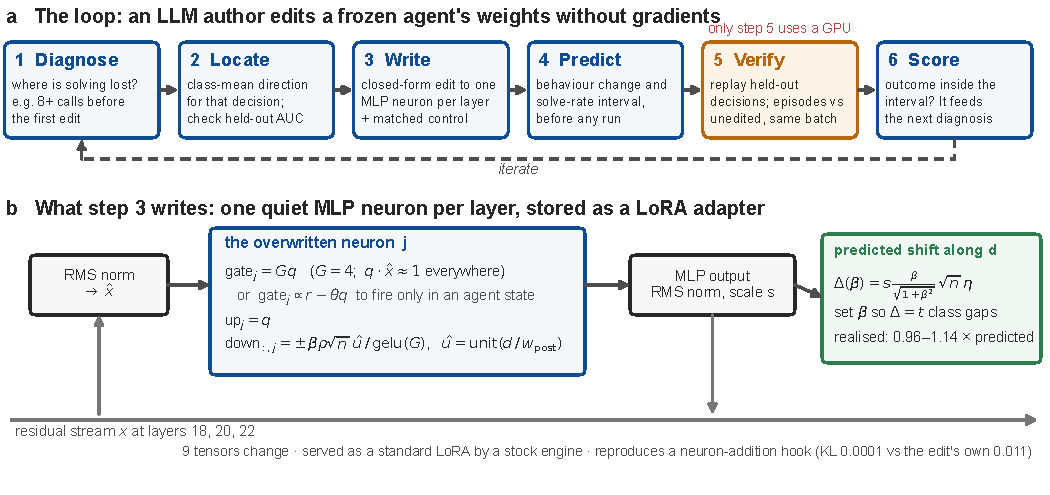
\includegraphics[width=1.0\linewidth]{figures/fig1_loop.pdf}
\end{center}
\caption{\textbf{The method.} (a) The loop of this paper. An LLM author diagnoses a failure from logged episodes of a frozen Gemma 4 E4B coding agent and locates a direction for the decision involved. It writes a closed-form edit and a matched random control and writes down its prediction. It verifies the edit against the unedited model in the same batch and scores the prediction. No step computes a gradient; only verification uses a GPU. (b) The edit of step 3. In each of three layers, the quietest MLP neuron is overwritten. The new neuron fires at a constant level (or only in a chosen agent state) and writes along the direction $d$. Eq.~(\ref{eq:shift}) predicts the shift, and the build measures it.}
\label{fig:loop}
\end{figure}

This paper delivers cheap, precise, verifiable control of a coding agent's decisions by LLM-written weight edits, and a measured account of when such control does and does not raise solve rate. We credit the idea of LLM-written weights to the two works above. Four things differ here. First, the target is a decision of a multi-step agent, not a single-turn output. Second, edits are gated on agent state instead of adding a constant direction; for example, one gate fires before the episode's first edit, with measured leakage elsewhere (\S\ref{sec:control}). Third, each edit carries a written prediction that we score afterwards. Fourth, we compare three LLM authors under one brief. We ask three questions. Does an edit move a named decision where a matched random control does not? Does it raise the solve rate beyond its control? How often is the author's written prediction right?

\noindent Contributions, in order of the paper:
\begin{itemize}
    \item \textbf{Method} (\S\ref{sec:method}): to our knowledge the first LLM-authored weight edits for a multi-step coding agent, gated on agent state, sized in closed form and packed exactly into a LoRA~\citep{Hu2021LoraLowrank} adapter that a stock engine serves.
    \item \textbf{Decision control} (\S\ref{sec:control}): always-on edits move three decisions with a dose-response on held-out decisions, while matched random controls stay near the unedited value.
    \item \textbf{Solve rate} (\S\ref{sec:devgain}--\ref{sec:heldout}): the best edit solved 30.3 against 25.3 tasks ($p = 0.014$ uncorrected); it does not survive Holm correction, and the pre-registered held-out test agreed in sign ($+3.0$, $p = 0.50$).
    \item \textbf{Diagnosis and evaluation lessons} (\S\ref{sec:diagnosis}, \S\ref{sec:negative}, \S\ref{sec:discussion}): a small coding agent fails by inconsistency, not incapacity, and solve rate is governed by run-to-run variance and selection.
    \item \textbf{Three-author benchmark} (\S\ref{sec:arena}): twelve edits and three controls from Claude, GPT and Gemini, each with a written 80\% interval scored afterwards.
\end{itemize}
We release the edit builder, an episode and decision dataset with labelled activations, and the three authors' prediction files as a reusable resource, together with all edits, pre-registrations and per-task results.


\section{Related Work}
\label{sec:related_work}
\textbf{LLM-authored weights.} \citet{Takehi2026SparksWeightspace} coined weight-space programming and report gains on a 0.8B model. The closest prior work is \citet{Bennington2026GradientfreeWeight}. They cut thinking tokens in Qwen3.8-27B with rank-one edits and test against a norm-matched orthogonal random control, which we adopt (TACT~\citep{Sui2026TactMitigating} also reports one). Both evaluate their edits on single-turn benchmarks. \citet{Mehta2026InterpretableWeightspace} have an LLM agent write the weights of small transformers and brain encoding models from scratch. The agent does no gradient training; a fixed evaluator fits the encoding models' linear read-out. They audit each saved model for interpretability. Their models are built whole for a fixed evaluator. We make sparse closed-form edits to a pretrained 4B-parameter agent, each with a written prediction and a matched random control, and evaluate whole agent episodes. We keep the idea of Takehi et al.\ and Bennington et al.\ and the latter's control; \S\ref{sec:intro} lists what we change.

% Comparison with closest prior work. Every cell is sourced in related_table_sources.md.
\begin{table}[t]
\centering
\small
\caption{How this work differs from the closest prior work. \emph{Cond.}: the change depends on a condition read from the hidden state. \emph{Plain weights}: the change is an ordinary weight tensor, servable by a stock engine without hooks. \emph{Control}: a random-direction or random-vector control reported. \emph{Agents}: evaluated on multi-step agent episodes. \emph{Author}: who produces the change (``contrast'': a direction from activation contrasts on human-chosen data, with layer and strength set by the authors). $^a$Random vectors of similar magnitude, qualitative and KL comparison. $^b$TACT-Gate and TACT-Cap; TACT-Add is unconditional. $^c$The rank-one update responds to the subject's key vector. $^d$For the three unconditional edits (\S\ref{sec:control}--\ref{sec:devgain}); in the benchmark each author built its own random control (Claude's is ungated and smaller than its gated edits; GPT's omits the rank-two rotation). $^e$For brain encoding the agent writes the feature network and a fixed evaluator fits a ridge read-out. $^\dagger$Dense weights edited in place are plain weights by construction; the source does not report serving them.}
\label{tab:related}
\resizebox{\linewidth}{!}{%
\begin{tabular}{@{}lllllll@{}}
\toprule
Work & Lives in & Cond. & Plain weights & Control & Agents & Author \\
\midrule
ActAdd~\citep{Turner2023SteeringLanguage} & Hook & No & No & Random vector$^a$ & No & Human (contrast) \\
CAA~\citep{Panickssery2023SteeringLlama} & Hook & No & No & No & No & Human (contrast) \\
CAST~\citep{Lee2024ProgrammingRefusal} & Hook & Yes & No & No & No & Human (contrast) + grid search \\
TACT~\citep{Sui2026TactMitigating} & Hook & Yes$^b$ & No & Norm-matched random & Yes & Human (contrast) \\
ROME~\citep{Meng2022LocatingEditing} & Weights & Key$^c$ & Yes$^\dagger$ & No & No & Optimisation + closed form \\
\citet{Arditi2024RefusalLanguage} & Weights & No & Yes$^\dagger$ & No & No & Human (contrast) \\
\citet{Takehi2026SparksWeightspace} & Weights & No & Yes$^\dagger$ & No & No & LLM author \\
\citet{Bennington2026GradientfreeWeight} & Weights & No & Yes & Norm-matched random & No & Human (contrast) \\
\citet{Mehta2026InterpretableWeightspace} & Weights (whole small model)$^e$ & n/a & n/a & Interpretable baselines & No & LLM author \\
\midrule
This paper & Weights (LoRA) & Yes (gate) & Yes (vLLM) & Norm-matched random$^d$ & Yes & LLM author \\
\bottomrule
\end{tabular}%
}
\end{table}


\textbf{Activation steering.} Steering methods add a direction to the residual stream at inference. Activation addition~\citep{Turner2023SteeringLanguage}, contrastive activation addition~\citep{Panickssery2023SteeringLlama} and representation engineering~\citep{Zou2023RepresentationEngineering} obtain the direction from contrasting prompts, as we do. Inference-time intervention~\citep{Li2023InferencetimeIntervention} and in-context vectors~\citep{Liu2023IncontextVectors} are close variants. Conditional activation steering~\citep{Lee2024ProgrammingRefusal} applies a steering vector only when a condition direction is present in the hidden state. It is the inference-time counterpart of our gate. ReFT~\citep{Wu2024ReftRepresentation} learns such interventions by training. AxBench~\citep{Wu2025AxbenchSteering} finds that prompting beats representation-based steering and that difference-of-means is the strongest concept detector. TACT~\citep{Sui2026TactMitigating} steers coding agents along overthinking and overacting axes and reports gains of 4.8--5.8 points. \citet{Silva2026LatentProgramming} show that linear probes on a coding agent's hidden states forecast whether its pending edits will succeed. Our probe for patch correctness (\S\ref{sec:negative}) is a signal of the same kind. All of these methods need hooks or extra modules in the inference stack. We compile the direction and its condition into existing weights, because the competition scores submitted weights served by a stock engine (\S\ref{sec:primitive}).

\textbf{Direct weight editing.} ROME~\citep{Meng2022LocatingEditing} and MEMIT~\citep{Meng2022MasseditingMemory} change factual associations with closed-form updates to MLP weights. \citet{Arditi2024RefusalLanguage} remove a refusal direction by orthogonalising weights against it. These edits remove or replace what existing weights write. Our primitive adds a new write by repurposing a neuron that contributes almost nothing, and it targets a recurring agent decision.

\textbf{Small trained changes and agent training.} Deletion Tuning~\citep{Lu2026SurprisingEffectiveness}, BitFit~\citep{Benzaken2021BitfitSimple} and task arithmetic~\citep{Ilharco2022EditingModels} change few weights but obtain the change by training. Our edits and our one-shot deletion experiment (\S\ref{sec:negative}) use no optimisation step. For software agents, SWE-bench~\citep{Jimenez2023SwebenchCan} defines the task, and SWE-agent~\citep{Yang2024SweagentAgentcomputer} defines an agent--computer interface for it. SWE-Gym~\citep{Pan2024TrainingSoftware}, R2E-Gym~\citep{Jain2025R2egymProcedural} and SWE-smith~\citep{Yang2025SwesmithScaling} improve agents by training on executable repository environments. SWE-Gym uses real environments; R2E-Gym and SWE-smith synthesise them.

\section{Method}
\label{sec:method}
\subsection{Setting}
\label{sec:setting}
\textbf{Model and agent.} The model is Gemma 4 E4B~\citep{Team2026Gemma4}: 42 layers, residual width $n = 2560$, MLP width 10240, activation \texttt{gelu\_pytorch\_tanh}. We use its INT4 quantisation-aware checkpoint, served with vLLM. The agent calls six tools: run a command, read, edit and write a file, status, and submit. It uses greedy decoding, a thinking budget of 2,560 tokens, at most 34 tool calls and 7.5 minutes per episode. A task is solved when hidden tests pass. We edit the released base model (the \emph{unedited model}) and, in three experiments, our wave-5 RL adapter.

\textbf{Tasks and what is in-sample.} The 170 \emph{development tasks} are 106 competition-format tasks and 64 SWE-rebench~\citep{Badertdinov2025Swerebench} tasks. The SWE-rebench repositories are disjoint from all RL training pools. The 130 \emph{held-out tasks} come from 78 repositories. These share no repository with the development tasks and never appeared in the logs that we computed directions from (\S\ref{sec:heldout}). The diagnosis (\S\ref{sec:diagnosis}) used episodes of the 170 development tasks. We split logged decisions into training and held-out sets by episode, not by task. Development gains are therefore in-sample at the task level. The 130 held-out tasks are the out-of-sample test of solve rate.

\textbf{What each data split is used for.} The training split of logged decisions from development-task episodes fits directions and read-outs. The held-out split of those decisions (by episode, same tasks) checks direction AUC, sizes gated edits, measures realised shifts, and supports decision replay. Replay on this split therefore measures in-distribution control. The 170 development tasks serve diagnosis, agent evaluation, and the choice of strengths and of edits to repeat. The 130 held-out tasks serve only the two pre-registered tests.

\textbf{Unit of comparison.} An \emph{arm} is one model variant (the unedited model, an edit or a control) evaluated on every task. Greedy runs of this stack are not repeatable. A \emph{batch} is one run of every arm on all tasks at once. vLLM loads the base checkpoint and serves every arm as a LoRA module; the unedited model is an all-zero adapter. Each arm has its own evaluator process. The arms share one continuous-batching queue, so a request's batch neighbours vary between runs. Two copies of the unedited model in the same held-out run differed by 11.7 tasks-equivalent (\S\ref{sec:heldout}). We therefore make every comparison within one batch, against the unedited arm served alongside the edit. Every batch includes the unedited model. The primary unit of analysis is the batch. We report the mean per-batch difference in solved tasks with a 95\% $t$ confidence interval (CI) and a two-sided paired $t$ test over batches. Task-level tests (per-task differences summed over batches) are secondary, and we label them as such.

\subsection{Locating a direction}
\label{sec:locate}
A binary label on logged decision points defines a direction. For ``explore more before editing'', the label is whether the next tool call makes the episode's first edit (class 1) or explores further (class 0). The position is the first generated token of that call. We record the layer outputs at these positions for 400 training and 160 held-out decisions per class. For layer $l$, the direction $d_l = \mu_1 - \mu_0$ is the difference of the class means of the layer output on the training split. Its norm $\lVert d_l \rVert$ is the \emph{class gap}. We use this single split, without further regularisation or cross-validation. We keep a direction if projecting held-out decisions onto $d_l$ separates the classes, measured as AUC. For explore-more, the AUC is 0.77, 0.81 and 0.83 at layers 18, 20 and 22, the three layers we write. To make the agent explore more, we write $-d_l$.

\subsection{The primitive: a hand-written neuron}
\label{sec:primitive}
\textbf{Why weights and not a hook.} The competition scores a submitted checkpoint served by a stock inference engine. An intervention must therefore live in the weights; an activation hook cannot be submitted. Gemma 4 has no bias terms, so we must also build a constant shift from the input. In the MLP of layer $l$, with $\hat{x} \in \mathbb{R}^n$ the normalised MLP input, neuron $j$ computes
\begin{equation}
\label{eq:neuron}
    a_j = \gelu(\mathrm{gate}_j \cdot \hat{x}) \, (\mathrm{up}_j \cdot \hat{x}), \qquad y = \sum_j \mathrm{down}_{:,j} \, a_j, \qquad h_{\mathrm{out}} = s_l \left( x + w_{\mathrm{post}} \odot y / \mathrm{rms}(y) \right),
\end{equation}
where $\mathrm{gate}_j$ and $\mathrm{up}_j$ are rows of the two input projections, $\mathrm{down}_{:,j}$ is a column of the output projection, $w_{\mathrm{post}} \in \mathbb{R}^n$ is the weight of the output normalisation, $s_l$ is the layer's output scalar, $x$ is the residual input and $\odot$ is the elementwise product. The MLP output is RMS-normalised, so only its direction matters.

\textbf{Read.} We fit a ridge read-out $q$ with target 1, so that $q \cdot \hat{x} \approx 1$ at every position. The fit uses relative penalty $10^{-3}$, the dual form, and the 3,998 training-split positions (about five per training decision call). On held-out positions, $q \cdot \hat{x}$ has mean 0.98--0.99 and standard deviation (SD) 0.02--0.04 across the three layers for the always-on edit (other builders: Appendix~\ref{app:gated}).

\textbf{Neuron choice.} In each layer we overwrite the neuron with the smallest product of mean absolute activation and down-column norm (0.22--0.32 of the layer median). Overwriting it removes almost nothing.

\textbf{Write.} The overwritten neuron gets
\begin{equation}
\label{eq:write}
    \mathrm{gate}_j = G\, q, \qquad \mathrm{up}_j = q, \qquad \mathrm{down}_{:,j} = \pm\,\beta \, \rho \, \sqrt{n} \; \hat{u} \, / \, \gelu(G), \qquad \hat{u} = \unit(d_l / w_{\mathrm{post}}),
\end{equation}
with gain $G = 4$, $\rho$ the mean RMS of the natural MLP output $y$ on training positions, $\unit(v) = v / \lVert v \rVert$, the division elementwise, and the sign chosen by the author. The neuron fires at $a_j \approx \gelu(G)$ everywhere. It adds a vector of norm $\beta \rho \sqrt{n}$ along $\hat{u}$, which is $\beta$ times the norm of the natural output. The map $d_l \mapsto \hat{u}$ undoes the output normalisation: $w_{\mathrm{post}} \odot \hat{u} = \eta\, d_l / \lVert d_l \rVert$ with $\eta = \lVert w_{\mathrm{post}} \odot \hat{u} \rVert$.

\textbf{Predicted shift and the strength scale.} Assume the natural output $y$ is orthogonal to $\hat{u}$ and has RMS $\rho$. Then $y + \beta \rho \sqrt{n}\, \hat{u}$ has RMS $\rho \sqrt{1+\beta^2}$, and the full change of the layer output is
$\Delta h = s_l \big[ \tfrac{\beta \sqrt{n}}{\sqrt{1+\beta^2}}\, w_{\mathrm{post}} \odot \hat{u} - \big(1 - \tfrac{1}{\sqrt{1+\beta^2}}\big)\, w_{\mathrm{post}} \odot y / \rho \big]$.
The second term shrinks the natural write by $1 - 1/\sqrt{1+\beta^2} \approx \beta^2/2$. This is 0.04--1.2\% for the $\beta$ of strengths up to 0.25 and 14.3\% at the cap $\beta = 0.6$ (Appendix~\ref{app:params}). Eq.~(\ref{eq:shift}) keeps only the first term. It ignores the part of the natural write that already lies along $d_l$; the shrinkage acts on that part too, so at layer 22 at the cap the natural write's component along $d_l$ also shrinks by 14\%. Also, because $\hat{u} \propto d_l / w_{\mathrm{post}}$, the pre-normalisation inner product $y \cdot \hat{u}$ weights each coordinate of $(w_{\mathrm{post}} \odot y) \cdot d_l$ by $1/w_{\mathrm{post}}^2$. Orthogonality of $y$ and $\hat{u}$ therefore makes $w_{\mathrm{post}} \odot y$ and $w_{\mathrm{post}} \odot \hat{u}$ orthogonal only when $w_{\mathrm{post}}$ is constant. Under these approximations, the layer output moves along $d_l / \lVert d_l \rVert$ by
\begin{equation}
\label{eq:shift}
    \Delta_l(\beta) = s_l \cdot \frac{\beta}{\sqrt{1+\beta^2}} \cdot \sqrt{n} \cdot \eta .
\end{equation}
This predicted shift is the projection of the change in $h_{\mathrm{out}}$ onto the unit direction. We report it in units of the class gap. An edit of \emph{strength} $t$ sets $\beta$ per layer so that $\Delta_l(\beta) = t\, \lVert d_l \rVert$. With $\kappa = t \lVert d_l \rVert / (s_l \sqrt{n}\, \eta)$, this gives $\beta = \kappa / \sqrt{1 - \kappa^2}$, capped at 0.6. Strength 0.25 gives $\beta = 0.057$, 0.060 and 0.154 at the three layers (Appendix~\ref{app:params}). The layer scalar enters through $\kappa$. At layer 22 ($s_{22} = 0.173$), $\kappa = 0.61\,t$. The shift therefore saturates at $t \approx 1.64$ ($\kappa = 1$), and the cap binds from $t \approx 0.84$ (layers 18 and 20: from $t \approx 2.1$--2.3). We measure the realised shift on held-out positions wherever a build report records it. The prediction holds closely for always-on edits. Over 12 edit--layer pairs built by Claude and Gemini, the realised shift is 0.96--1.14 times Eq.~(\ref{eq:shift}) (mean 1.06). For gated edits, the ratio is the realised shift averaged over held-out gate-ON positions, divided by Eq.~(\ref{eq:shift}) at the builder's recorded $\beta$. This ratio follows how strongly the gate fires there: 0.92--1.17 per unit of firing over 13 GPT and Gemini pairs (\texttt{scripts/shift\_check.py}). The raw ratio ranges from 0.64--0.71 for Claude's early-calls gate to 2.14 for a Gemini guard that fires at twice its reference level. For Claude's gates, the realised value is the bisection target itself. For the early-calls gate, this target is 0.3 gaps, averaged over all its held-out ON positions, where its mean activation is 2.0--2.2 of the 4.0 of full firing. The decision token of calls up to 4 moves more (Appendix~\ref{app:gated}).

\textbf{Gated neuron.} A gated edit fires only where a read direction for an agent state is present. Its gate row combines a read-out $r$ for the gating label with the constant read-out, $\mathrm{gate}_j \propto r - \theta q$. The pre-activation is therefore about $+G$ where the state is present and negative elsewhere. At negative pre-activations $\gelu$ is near zero but not zero. \texttt{gelu\_pytorch\_tanh} is negative on $(-3, 0)$, with minimum $-0.17$ at $-0.75$. A weakly negative pre-activation therefore writes up to 4\% of a full firing with reversed sign. \S\ref{sec:control} measures how often the gate fires outside its fit. The gated edits of the benchmark fit $r$ by ridge regression. They size the write by measurement on the held-out split instead of Eq.~(\ref{eq:shift}), so their sizing is in-sample for that split. Appendix~\ref{app:gated} gives these details and the other authors' rotation and attention edits. A neuron edit in three layers changes nine tensors: one gate row, one up row and one down column per layer. We store it as a LoRA update, exact up to bf16 rounding.

\textbf{Matched random control.} The control overwrites the same neurons with the same gate row and up row. We build its write direction in residual space. We take $d_l$ with a random sign per dimension and make it orthogonal to $d_l$ by Gram--Schmidt. We then map it through $1 / w_{\mathrm{post}}$ and normalise it to unit length, so the down column has the same norm as the edit's. Its cosine with $d_l$ is zero, and its size in the residual stream is 0.99--1.04 of the edit's per layer. This strict construction applies to the unconditional edits of \S\ref{sec:control}--\ref{sec:devgain}. In the three-author benchmark, each author built its own control (Appendix~\ref{app:gated}).

\textbf{The compiled edit closely reproduces the intended intervention.} We compare the adapter as served with an inference-time hook that adds the same neuron write to the MLP output. Both run teacher-forced through a twin of the serving numerics (INT4 weights, bfloat16) on 76 held-out decision calls. We test the always-on explore-more edit and the before-first-edit gate. Relative to the unedited model, the residual-stream changes of adapter and hook have cosine 0.972--0.992 and 0.984--0.996 across eight layers from 18 to 41. Their norm ratios are within 0.4\% of 1. Over completion tokens, KL(hook$\,\Vert\,$adapter) is $1.1\times10^{-4}$ and $1.2\times10^{-4}$. This is 99 and 110 times smaller than the edit's own effect, KL(unedited$\,\Vert\,$adapter) $= 0.011$ and $0.013$. At the decision token itself, KL(unedited$\,\Vert\,$adapter) is $3.4\times10^{-5}$ for both edits (Appendix~\ref{app:hook}). Most of the measured effect is therefore on completion tokens after the decision. A plain vector addition matches less closely (cosine 0.80 and 0.73 at layer 22; Appendix~\ref{app:hook}).

\subsection{The loop and the written-prediction protocol}
\label{sec:loop}
Figure~\ref{fig:loop} shows the loop. Algorithm~\ref{alg:loop} (Appendix~\ref{app:params}) lists its six steps: diagnose, locate, write, predict, verify by replay and by agent evaluation, and score. The author is an LLM with shell access to the model weights, stored activations and logged episodes. Steps 1--4 run on a CPU; only verification uses a GPU.

\textbf{Prediction protocol.} Step 4 produces a file that is fixed before step 5 starts. In the three-author benchmark (\S\ref{sec:arena}), each edit's entry has the fields \texttt{diagnosis}, \texttt{mechanism}, \texttt{predicted\_behaviour} and \texttt{predicted\_solved\_delta}. The last field holds a point value and an 80\% interval in solved tasks out of 170, relative to the unedited model of the same batch. A prediction is a hit when the first measured difference falls inside the interval.

\section{Experiments}
\label{sec:experiments}
\subsection{Diagnosis: where the solve rate is lost}
\label{sec:diagnosis}
The diagnosis supplies the behaviours that later edits target. It is observational: every odds ratio is a within-task (Mantel--Haenszel) association. The authoring model first computed the edit-failure and calls-before-first-edit tallies. We then recomputed them from the saved trajectories with our own code (\texttt{diag\_recompute}). Every reported value reproduces, with two episodes moved between groups (Appendix~\ref{app:diag}).

\begin{itemize}
    \item \textbf{The model is inconsistent, not incapable.} Evaluation is greedy. Yet over the 13 unedited runs of batches 3--15, a single run solves 22--30 tasks, 51 different tasks are solved at least once, and 9 are solved in every run.
    \item \textbf{Failed edits go with lost episodes.} In those 13 runs (2,210 episodes), 35\% of 4,916 \texttt{edit\_file} calls fail (1,727). Episodes with no failed edit are solved 21\% of the time (318 of 1,538). Episodes with at least one failed edit are solved 4\% of the time (24 of 672). The within-task odds ratio of solving given any failed edit is 0.42 (95\% CI 0.23--0.74). If we also count the 165 edit calls that the harness rejected before running, 38.5\% fail and the odds ratio is 0.44.
    \item \textbf{Long exploration loses episodes.} Over the same 2,210 episodes, 17\% of episodes make 8 or more calls before the first file edit. Within task, these episodes solve far less than the task's other episodes (odds ratio 0.12, 95\% CI 0.04--0.38). We bin the 6 episodes that never edit a file by their total calls; three fall in 8+, all unsolved. On the 2,204 episodes with at least one file edit, the 8+ odds ratio is unchanged (0.12, CI 0.04--0.37; \texttt{dr\_fix/m4\_8plus\_edited\_only.py}). Episodes that never edit therefore do not drive it. The other bins have intervals that include 1 (0--2 calls 0.76, CI 0.39--1.48; 3--4 calls 1.42, 0.86--2.35; 5--7 calls 1.72, 0.97--3.06; Figure~\ref{fig:invu}). Raw solve rates are highest for 0--2 calls, because the model edits easy tasks quickly. Each bin draws on 19 to 36 informative tasks, because most tasks are never solved.
    \item \textbf{Reading before editing.} On the three unedited runs of batches 3--5 (510 episodes, 7 informative tasks), reading a file before the first edit shows no association with solving (odds ratio 1.0). Pooled over all 2,720 episodes of those batches (the 16 runs of the 170 tasks in the scripted per-episode file, edited arms included; the other runs of those batches are not in it), episodes that read first were solved more often (371 of 2,259 against 38 of 461; odds ratio 3.1, $z = 4.5$, 51 tasks with both outcomes and both conditions). This pooled association comes from the edited arms. Claude's later tally found no monotone benefit of longer exploration (Appendix~\ref{app:diag}).
\end{itemize}

\begin{figure}[t]
\begin{center}
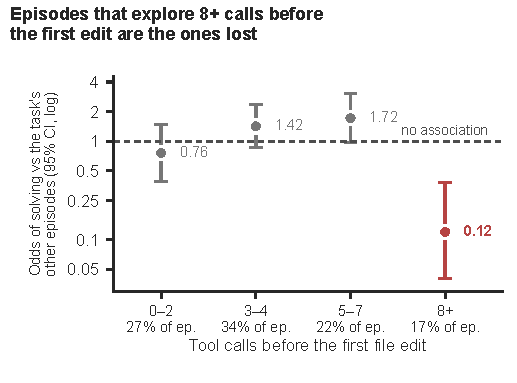
\includegraphics[width=0.5\linewidth]{figures/fig5_invu.pdf}
\end{center}
\caption{\textbf{Long exploration before the first edit is where episodes are lost.} Within-task Mantel--Haenszel odds ratio of solving for episodes in each bin of tool calls before the first file edit, against the task's other episodes; 13 unedited runs, 2,210 episodes; 95\% Robins--Breslow--Greenland intervals, log scale. Only the 8+ bin (red) excludes 1. The 6 episodes with no file edit are binned by their total calls; without them the 8+ odds ratio is 0.12 (0.04--0.37). Observational.}
\label{fig:invu}
\end{figure}

\subsection{Edits control decisions}
\label{sec:control}
\textbf{Claim tested:} an edit moves its targeted decision monotonically with its strength, and a matched random control of the same size does not.

\textbf{Setting.} For each edit, we regenerate held-out logged decisions once, greedily, and count the targeted decision. We do this under the unedited model, the edit at three strengths, and a matched random control. Intervals are Wilson 95\% intervals for proportions. We write the submit-sooner edit on the wave-5 RL adapter. Its submit-versus-keep-testing direction has held-out AUC 0.72--0.75 at the three written layers. We write the think-briefly and explore-more edits on the base model. This replay covers the always-on edits. For the gated edits of \S\ref{sec:arena}, we measured static per-position shifts (below) and teacher-forced comparisons (Appendix~\ref{app:hook}).

\begin{figure}[t]
\begin{center}
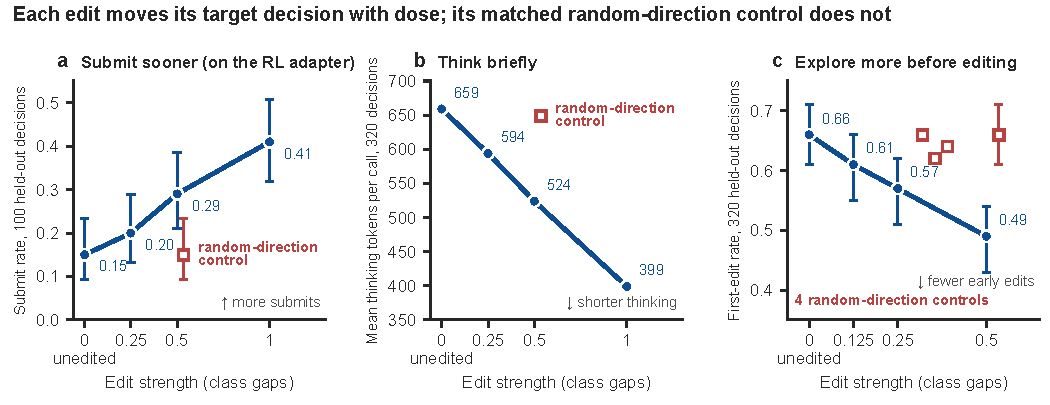
\includegraphics[width=1.0\linewidth]{figures/fig2_dose.pdf}
\end{center}
\caption{\textbf{Edits control decisions with dose; matched controls do not.} Replay of held-out logged decisions under the unedited model (strength 0), the edit at three strengths (blue) and matched random-direction controls (red squares, same neurons and norm). (a) Submit rate over $n = 100$ decisions, edit written on the RL adapter. (b) Mean thinking tokens per call over $n = 320$ decisions (means only; one control seed, matched to strength 0.5). (c) Rate at which the next call makes the episode's first edit, $n = 320$; four control adapters, one matched to strength 0.5 and three seeds matched to 0.25. Bars: Wilson 95\% intervals.}
\label{fig:dose}
\end{figure}

\textbf{Result.} Figure~\ref{fig:dose} and Table~\ref{tab:dose} (Appendix~\ref{app:params}) show a monotone dose-response for all three edits. The submit rate rises from 0.15 to 0.41; the control gives 0.15. Thinking tokens fall from 659 to 399; the control gives 649. The rate at which the next call makes the first edit falls from 0.66 to 0.49. The four control adapters give 0.66, 0.62, 0.64 and 0.66. The unedited rate was 0.64 to 0.66 in three separate replay runs, so replay noise is about 0.02. At the lowest strength (0.125; rate 0.606), the edit does not separate from the controls; one control seed gives 0.616. The effect carries from single decisions to whole episodes. The submit-sooner edit lowers mean tool calls per episode from 20.8 to 14.2 at strength 0.5 and to 8.8 at strength 1.0. Its 0.5-matched control gives 19.8 (one agent run per arm).

\textbf{Off-target effects.} Each edit also moves other statistics. Think-briefly at strength 1.0 lowers the first-edit rate from 0.64 to 0.52. At strength 0.5 it gives 0.60, the same as its 0.5-matched random control (0.60). Submit-sooner at strength 1.0 lowers thinking tokens per call from 282 to 167 (strength 0.5: 238; its 0.5-matched control: 288).

\textbf{Locality of gated edits.} The gated edits of \S\ref{sec:arena} allow a per-position check. We compute it from the stored bf16 tensors on held-out positions. Claude's before-first-edit gate reads its condition with held-out AUC 0.993--0.996. It fires on 85--88\% of positions before the first edit and on 1.2--1.4\% of its OFF positions (positions after the first edit that were in its fit). The shift along the explore direction is $-0.22$ to $-0.32$ class gaps before the first edit and 0.000 at decision positions after it. At prompt positions after the first edit, which were not in its fit, the shift is $-0.19$ to $-0.21$ class gaps (early-calls gate: $-0.08$ to $-0.12$). The gate thus also acts on these prompt positions. Appendix~\ref{app:gated} gives the other gates.

\textbf{Episode cost.} Submit-sooner shortens episodes by design. The explore-more edits do not reduce episode cost relative to the unedited model (Appendix~\ref{app:negative}, Table~\ref{tab:cost}).

\subsection{Always-on explore-more on development tasks}
\label{sec:devgain}
\textbf{Claim tested:} writing ``explore more before editing'' at every position raises solved development tasks at low strength and lowers them at high strength.

\textbf{Setting.} Batches 3--15 each ran eight to eleven arms, the unedited model included (schedule in Appendix~\ref{app:schedule}). We compare every edit with the unedited model served alongside it in the same batch. In batches 3--5, we compare edits written on the RL adapter with that adapter (Appendix~\ref{app:repro}). Twelve of the 13 batches have an explore-more arm. We chose strengths on these tasks and later pre-registered strength 0.25 for the held-out test. The pool of strengths 0.125--0.5 is a post hoc summary. ``Gained / lost'' counts tasks that the arm solves and the unedited model of the same batch does not, and the reverse, summed over runs.

\begin{table}[t]
\caption{Always-on explore-more on the base model, 170 development tasks. $\Delta$ is the mean difference in solved tasks against the unedited model of the same batch, with a 95\% $t$ CI and two-sided paired $t$ test. For the edit rows the unit is the run; for the control row the 14 runs are first averaged within each of their 7 batches ($n = 7$); its Mean is the average of these batch means (25.8; the mean over the 14 runs is 25.6). ``Unedited, same batches'' is the mean of the unedited model over the batches of that row. The pooled row averages the 0.125--0.5 arms within each of 12 batches (post hoc). In batches 3--5 the base-model arms and the RL-adapter arms ran as two separate groups; every row here uses base-model arms and the unedited arm of the same group. Rows with different strengths come partly from different batches, so the within-batch comparison is the one in batches 6, 7 and 10 given in the text.}
\label{tab:explore}
\centering
\footnotesize
\setlength{\tabcolsep}{3.5pt}
\resizebox{\linewidth}{!}{\begin{tabular}{lrlrrrlrr}
\toprule
Arm & Runs & Solved per run \up & Mean \up & Unedited, same batches & $\Delta$ \up & 95\% CI & $p$ & Gained / lost \\
\midrule
Unedited model & 13 & 22--30 & 26.3 & & & & & \\
Explore-more 0.125 & 4 & 31, 30, 28, 33 & 30.5 & 26.0 & $+4.5$ & [$-0.3$, $+9.3$] & 0.058 & 40 / 22 \\
Explore-more 0.25 & 7 & 32, 29, 30, 31, 29, 26, 27 & 29.1 & 25.1 & $+4.0$ & [$+0.3$, $+7.7$] & 0.040 & 75 / 47 \\
Explore-more 0.5 & 10 & 28, 31, 33, 30, 26, 32, 30, 24, 28, 27 & 28.9 & 26.2 & $+2.7$ & [$-0.3$, $+5.7$] & 0.074 & 98 / 71 \\
Explore-more 1.0 & 1 & 18 & 18.0 & 24.0 & $-6.0$ & & & 8 / 14 \\
Pooled 0.125--0.5 & 12 batches & & 28.8 & 26.2 & $+2.7$ & [$+0.3$, $+5.0$] & 0.030 & \\
Matched random controls & 14 & 23--28 & 25.8 & 25.9 & $-0.04$ & [$-3.1$, $+3.0$] & 0.98 & 116 / 117 \\
\bottomrule
\end{tabular}}
\end{table}

\textbf{Result.} In Table~\ref{tab:explore} (per-run counts: Figure~\ref{fig:solve}, Appendix~\ref{app:negative}), the gain shrinks as strength grows from 0.125 to 0.5. These rows cover different batches. In the three batches that ran all three strengths together (6, 7 and 10), the means are 29.7, 30.0 and 31.0 for strengths 0.125, 0.25 and 0.5, against 25.7 for the unedited model: within a batch, the gain is flat across this range. The single run at strength 1.0 is 6 tasks below its unedited model. We average the edit arms at strengths 0.125--0.5 within each batch; this pooled quantity is distinct from the strength-0.5 row, which has the same $\Delta$. The pooled edit exceeds the unedited model by 2.7 tasks over 12 batches (95\% CI $+0.3$ to $+5.0$, $p = 0.03$; higher in 9 batches, sign test $p = 0.15$). It exceeds the mean of the random controls by 3.6 tasks in the 7 batches that contain both (CI $+2.2$ to $+5.1$, $p < 0.001$; higher in 7 of 7, sign test $p = 0.016$). The controls do not differ detectably from the unedited model in those batches ($-0.04$ tasks, 95\% CI $-3.1$ to $+3.0$). The pre-registered strength 0.25 alone exceeds the controls by 3.7 over 6 batches (CI $+2.1$ to $+5.3$, $p = 0.002$). It exceeds its own 0.25-matched controls by 3.3 over the 5 batches that contain them (CI $+1.3$ to $+5.2$, $p = 0.010$; \texttt{dr\_fix/exp\_checks.py}). The reversed sign (``edit sooner'') solved 12 at strength 1.0 and 22 at strength 0.5, against 28 for the unedited model in one batch.

\textbf{Replication trend and coverage.} The gain was $+4.3$ in the first six batches with an edit arm (4--9; $p = 0.07$) and $+1.1$ in the last six (10--15; CI $-1.2$ to $+3.4$, $p = 0.27$). Of the 170 tasks, 90 were never solved in any of the 109 complete runs of batches 3--15. In the 96 runs on the base model (excluding the 13 runs on the RL adapter), 94 were never solved. The edit therefore acts on reliability on tasks that the model can already solve.

\subsection{Three LLM authors, one brief}
\label{sec:arena}
\textbf{Claim tested:} the loop does not depend on one author; authors' written predictions of solve-rate change are calibrated; and an LLM-written edit raises solved development tasks over the unedited model and over its author's random control.

\textbf{Setting.} We gave one brief to three frontier LLMs, named here by their product names: Claude Fable 5.2, GPT Astra 6 and Gemini 4 Carbon. Each LLM author worked in a fresh session with shell access. The brief gave raw diagnosis rates: the share of failed edits, solve rates with and without a failed edit, the failure rate by edit index, and how episodes end. It also gave the always-on explore-more results and the solved counts of earlier edits. It contained no odds ratios and no calls-before-first-edit analysis (Appendix~\ref{app:diag}). Each author also received the stored activations and tools and 90 minutes of CPU-only wall time, with no access to evaluation. Claude computed the 13-run unedited-only analysis of \S\ref{sec:diagnosis} (2,210 episodes) during its own session; this analysis was not in the brief. An edit had to be a LoRA adapter of rank at most 32. Each author delivered four edits ranked by preference, a random control for its first choice, build scripts, and the prediction file of \S\ref{sec:loop}. Each author's five adapters ran in one \emph{screening batch} with the unedited model (batches 21--23). We then repeated four edits in \emph{replication batches} 24--28. Claude's two gates and GPT's gate + rotation ran in all five, and Gemini's edit ran in batches 25 and 27. Each repeated edit meets its own author's control in three or four batches in total (Appendix~\ref{app:schedule}). We chose the repeats after the screening batches; the replication-only columns exclude that selection.

\textbf{The authors converged.} The shared brief already reported the low-dose explore-more gains. Given that brief, all three authors gated or weakened explore-more instead of writing it at every position. Claude gated it on a ``before the first edit'' read-out. GPT gated it on the token position where a decision starts. Gemini paired a weak explore write (0.14 class gaps per layer, layers 18--22) with a concise-thinking write (0.12 class gaps, layers 24--28). GPT wrote the only rotation, and Gemini the only attention edit. \emph{Controls.} Claude's control is an \emph{ungated 0.125-gap control}: the random-direction counterpart of its always-on edit at 0.125 class gaps per layer, not orthogonalised to the explore direction. It is ungated and smaller than the gated edits it is compared with (0.25 and 0.30 class gaps). GPT's control omits the rank-two rotation. We did not run a gate- and norm-matched control (Appendix~\ref{app:gated}).

\begin{table}[t]
\caption{The four repeated edits on the 170 development tasks: mean per-batch difference in solved tasks ($\Delta$), 95\% $t$ CI and two-sided paired $t$ test over $n$ batches. ``All batches'' includes the screening batch that selected the edit; ``replication only'' excludes it. ``Edit $-$ control'' and ``control $-$ unedited'' use the batches shared with the author's own random control. With four shared batches a two-sided sign test cannot fall below $p = 0.125$. For Claude's two gates the control is its ungated 0.125-gap control, not a gate- and norm-matched one; GPT's control omits the rotation.}
\label{tab:arena}
\centering
\footnotesize
\setlength{\tabcolsep}{2.5pt}
\resizebox{\linewidth}{!}{\begin{tabular}{lrrlrrrlrrrlrrr}
\toprule
 & \multicolumn{3}{c}{Edit $-$ unedited, all} & & \multicolumn{3}{c}{Edit $-$ unedited, replication only} & & \multicolumn{3}{c}{Edit $-$ control} & & \multicolumn{2}{c}{Control $-$ unedited} \\
\cmidrule(lr){2-4}\cmidrule(lr){6-8}\cmidrule(lr){10-12}\cmidrule(lr){14-15}
Edit & $n$ & $\Delta$ \up & CI; $p$ & & $n$ & $\Delta$ \up & CI; $p$ & & $n$ & $\Delta$ \up & CI; $p$ & & $\Delta$ & $p$ \\
\midrule
Claude: before-first-edit gate & 6 & $+5.0$ & [1.6, 8.4]; .014 & & 5 & $+4.2$ & [0.5, 7.9]; .033 & & 4 & $+3.75$ & [$-$1.7, 9.2]; .11 & & $+1.75$ & .10 \\
Claude: early-calls gate & 6 & $+4.7$ & [1.2, 8.2]; .019 & & 5 & $+4.4$ & [$-$0.1, 8.9]; .054 & & 4 & $+3.5$ & [0.5, 6.5]; .035 & & $+1.75$ & .10 \\
GPT: decision-token gate + rot. & 6 & $+2.3$ & [$-$1.3, 5.9]; .16 & & 5 & $+2.0$ & [$-$2.6, 6.6]; .30 & & 4 & $+2.0$ & [$-$2.7, 6.7]; .27 & & $+0.5$ & .81 \\
Gemini: explore + concise & 3 & $+5.7$ & [$-$0.1, 11.4]; .051 & & 2 & $+5.0$ & [$-$20, 30]; .24 & & 3 & $+2.7$ & [$-$6.1, 11.4]; .32 & & $+3.0$ & .45 \\
\bottomrule
\end{tabular}}
\end{table}

\textbf{Development-set solve rate.} The unedited model solved 21--29 tasks across the eight batches (mean 25.25, SD 2.8). Claude's before-first-edit gate solved 33, 29, 31, 31, 30, 28 against 24, 27, 28, 22, 25, 26 for the unedited model beside it. That is 30.3 against 25.3 over these six batches, higher in all six (Table~\ref{tab:arena}; Figure~\ref{fig:arena} in Appendix~\ref{app:calib}; sign test $p = 0.031$). The gate had the largest screening-batch difference of the twelve edits ($+9$), and that batch is among the six. For scale, Gemini's random control gained $+8$ in its own screening batch. On the five replication batches alone, the gate solved 29.8 against 25.6 ($+4.2$, $p = 0.033$ uncorrected). Against Claude's ungated 0.125-gap control, the gate gained 3.75 over the four shared batches ($p = 0.11$). Over the three replication batches among them, it gained 2.3 (CI $-3.4$ to $+8.1$, $p = 0.22$). The control itself gained 1.75 over the unedited model ($p = 0.10$; higher in 4 of 4 batches). The early-calls gate is the only edit whose batch-level difference from its control has $p < 0.05$ ($+3.5$, $p = 0.035$, four batches). This compares a gate with a 0.30-gap target against the ungated 0.125-gap control. Replication-only, that difference is $+3.0$ over three batches ($p = 0.12$). Task-level tests agree in sign and are weaker against controls (Appendix~\ref{app:stats}).

\textbf{Multiple comparisons.} We correct each stage of the benchmark with Holm--Bonferroni over tests of one shape. Screening: every one of the twelve edits has one batch against the unedited model. There, the gate's task-level paired $t$ test gives $p = 0.020$, which becomes 0.24 after Holm, and every other edit's is at least 0.57; its exact McNemar $p = 0.035$ becomes 0.42 (\texttt{dr\_fix/exp\_checks.py}). Replication: over the four repeated edits on the replication-only batches, the gate's batch-level $p = 0.033$ becomes 0.13. No edit is significant after correction. (Holm over all twelve edits with their full batch sets, which mixes six-, three- and one-batch tests, takes the gate's task-level $p = 0.010$ to 0.12.) Task-level tests treat the batches as fixed, so their standard errors omit batch-to-batch noise (run-to-run SD 2.7--2.8 solved tasks); the batch-level $t$ test includes it. The pooled McNemar test for the gate gives $p = 0.002$ (Appendix~\ref{app:stats}). It treats 1,020 task--batch pairs as independent, although the same 170 tasks recur in every batch, so we read it as descriptive. We built a within-batch permutation null: per task, we swapped the labels of each edit arm and the unedited arm at random (10,000 permutations, seed 0). Under this null, the largest of the twelve screening differences has median $+7$ and 95th percentile $+11$. The gate's $+9$ is therefore within the selection null ($p = 0.22$; 0.18 under a joint permutation of all arms; 0.11 under a Gaussian model with the run-to-run SD of 2.7 over the 21 unedited runs). The test of the gate is thus the five replication batches, where the edit was fixed in advance. There it gains $+4.2$ per batch, with 48 task-runs gained and 27 lost. The task-level permutation $p$ is 0.018 (two-sided; one-sided 0.009), and the batch-level $t$ test gives $p = 0.033$ (\texttt{scripts/selection\_null.py}).

\textbf{Pass@$k$.} Decoding is greedy, so repeated runs differ only through non-repeatable serving. Pass@$k$ (unbiased estimator over runs) therefore measures run-to-run variability, not sampling diversity. Across the 21 complete unedited runs on the development tasks, pass@1 is 15.2\%, pass@10 29.0\% and pass@21 32.9\% (56 tasks solved at least once; 9 in every run). Over its six batches, the before-first-edit gate raises pass@1 from 14.9\% to 17.8\% ($+5.0$ tasks, paired bootstrap 95\% CI $+1.3$ to $+8.8$). It raises pass@3 by $+4.25$ ($-0.85$ to $+9.75$) and pass@6 by $+4.0$ ($-4$ to $+12$). The gain in tasks is similar at every $k$; the pass@1 interval alone excludes zero. Against its matched random controls, the always-on explore-more edit is ahead at every $k$ (pass@1 $+4.1$, CI $+1.6$ to $+6.8$; pass@14 $+10.7$, CI $+3.1$ to $+18.6$; 7 batches). \texttt{PASSK.md} in the repository gives the full tables.

\textbf{Calibration.} Twelve of 15 first-run outcomes fell inside the author's 80\% interval (Wilson 95\% interval for the hit rate: 0.55 to 0.93). GPT scored 5 of 5, Gemini 4 of 5 and Claude 3 of 5 (Appendix~\ref{app:calib}). Among the twelve edits (the other three adapters are controls), ten outcomes were inside. The intervals mainly capture run-to-run noise. A fixed interval of $\pm 6$ tasks around zero also covers 12 of the 15 outcomes (not the same twelve). Point predictions were small ($-0.5$ to $+3.8$), and the authors' intervals were 10 to 14 tasks wide on average. The five outcomes of an author share one unedited run, so the effective sample is closer to three clusters than to 15 outcomes, and the Wilson interval, which assumes independence, is optimistic. On the replication batches, the mean differences of the four repeated edits ($+4.2$, $+4.4$, $+2.0$ and $+5.0$) all fall inside their authors' 80\% intervals. Claude's two misses were its two gates, both under-predicted ($+9$ and $+6$ against upper bounds of $+6$ and $+5$).

\subsection{Two pre-registered held-out tests}
\label{sec:heldout}
\textbf{Claim tested:} the development-set gain of an edit transfers to tasks that played no part in building or selecting it. Neither test confirmed this claim.

\textbf{Design.} Both tests use the same 130 held-out tasks, three rollouts per task and arm (390 rollouts per arm), the same harness and greedy decoding. Greedy runs are not repeatable, so the three rollouts are replicates. We wrote the plan of each test before any agent run with the tested arms on these tasks, using adapters that were already built. We report differences in \emph{tasks-equivalent}: the difference in solved rollouts divided by three. Thus $+1$ tasks-equivalent is three more solved rollouts of 390. Tests are paired over the 130 tasks on per-task solved rollouts. The minimum detectable effect (MDE) is the difference detectable with 80\% power at two-sided $\alpha = 0.05$, given the measured SD of the per-task differences.

\begin{table}[t]
\caption{Held-out tests: solved rollouts of 390 per arm (130 tasks $\times$ 3). Arms are compared only within a group. In Test 1 the arms ran in two groups of three, each with its own separately served copy of the unedited model (the same weights).}
\label{tab:heldout}
\centering
\small
\resizebox{\linewidth}{!}{\begin{tabular}{llrrr}
\toprule
Test, group & Arm & Solved rollouts \up & Solve rate \up & Tasks solved $\ge$ once \up \\
\midrule
1, group 1 & Unedited model & 135 & 34.6\% & 70 \\
1, group 1 & Explore-more 0.25 (primary) & 136 & 34.9\% & 71 \\
1, group 1 & Matched random control & 139 & 35.6\% & 68 \\
\midrule
1, group 2 & Unedited model (second copy) & 170 & 43.6\% & 86 \\
1, group 2 & Explore-more 0.125 & 160 & 41.0\% & 84 \\
1, group 2 & Explore-more 0.5 & 166 & 42.6\% & 90 \\
\midrule
2 & Unedited model & 161 & 41.3\% & 82 \\
2 & Before-first-edit gate (primary) & 170 & 43.6\% & 89 \\
2 & Claude's ungated 0.125-gap control & 159 & 40.8\% & 80 \\
2 & Gemini's explore + concise edit & 163 & 41.8\% & 83 \\
\bottomrule
\end{tabular}}
\end{table}

\textbf{Test 1: always-on explore-more, strength 0.25.} The plan named the primary arm, two comparators (unedited model, matched random control) and a prediction: the edit beats both by 1 to 4 percentage points. The unedited model solved 34.6\% of rollouts. The edit gained 0.33 tasks-equivalent over it (95\% CI $-6.6$ to $+7.3$; $p = 0.92$; MDE 10.0 tasks-equivalent, 7.7 percentage points). It lost 1.0 to the control (CI $-8.0$ to $+6.0$, $p = 0.78$). The edit was better on 24 tasks and worse on 30 (sign test $p = 0.50$). Stratified by whether a rollout finished before the outage or was rerun (below), the edit's difference is $-0.33$ tasks-equivalent (exact McNemar $p = 1.0$), and edit minus control is $-0.67$ ($p = 0.92$). \emph{Not confirmed.} An outage forced reruns of 58\% of rollouts under a rule fixed before we looked at outcomes. The two copies of the unedited model, served side by side with the same weights, then differed by 11.7 tasks-equivalent ($p = 0.006$). We therefore compare each arm only with the unedited copy served alongside it (Appendix~\ref{app:prereg}).

\textbf{Test 2: Claude's before-first-edit gate.} The plan ran four arms side by side with one unedited copy. It named one primary test: gate minus unedited model, confirmed if $p < 0.05$ with a positive difference. The unedited model solved 41.3\% of rollouts. The gate gained 3.0 tasks-equivalent (95\% CI $-5.7$ to $+11.7$; $p = 0.50$; 45 tasks better, 36 worse, sign test $p = 0.37$; MDE 12.4 tasks-equivalent, 9.5 percentage points). Against Claude's ungated 0.125-gap control (the same control as on the development tasks), the gate gained 3.7 (CI $-4.7$ to $+12.0$, $p = 0.39$). Gemini's edit gained 0.7 over the unedited model ($p = 0.86$), and the control lost 0.7 ($p = 0.87$). The sign matches development; the registered test is \emph{not confirmed.}

\textbf{Pass@3.} At $k = 3$, the gate solves 89 of 130 held-out tasks at least once, against 82 for the unedited model ($+7.0$, CI $-6$ to $+20$) and 80 for its control ($+9.0$, CI $-3$ to $+21$). The two unedited copies of Test 1, with identical weights, differ by 16 tasks at pass@3 (CI $+3$ to $+29$).

\textbf{Power.} Each test detects a gain of about 10 to 12 tasks-equivalent of 130. This is roughly three times the development gain of the tested edit, scaled from 170 to 130 tasks. The pool set the size of 130: it is every task of the source set that passed the repository-disjointness rule (Appendix~\ref{app:prereg}). At the variance of Test 2, about 790 tasks give 80\% power for a gain of 5 tasks per 130. The held-out tasks are also easier for this model: the unedited model solved 41\% of rollouts in Test 2, against 15\% of development tasks per batch. The confidence intervals contain both zero and the development gain. The tests do not confirm the development gain, and they do not rule it out.

\subsection{What did not work}
\label{sec:negative}
\textbf{Claim tested:} control of a decision is enough to solve more tasks. It is not, for every direction other than explore-more. Appendix~\ref{app:negative} gives each attempt with its numbers. Solved counts are out of 170 development tasks, with one run per arm.

Submit-sooner moved behaviour as predicted. It solved 33, 26 and 27 at three strengths, against 36 for the RL adapter it was written on. Think-briefly solved 28, 28 and 25 against 29. A test-before-submitting edit on the RL adapter solved 17 against 30 for that adapter. A direction for ``the patch being submitted is right'' reaches a held-out AUC of 0.61--0.62, against 0.77--0.83 for the explore direction by the same method. Edits aimed at failed file edits left the share of well-formed regenerated edits unchanged (Appendix~\ref{app:negative}). Two written rules gave no gain as prompt text: 25, 29 and 30 for the first rule, the second and both, against 30 for the unedited model. Compiling them into weights reproduced 53\% and 41\% of their activation shift at rank 16, with no solve-rate gain. A one-shot weight deletion chosen by gradient scores without weight updates (after \citealp{Lu2026SurprisingEffectiveness}) scored below random deletions on one batch of 64 tasks.

A pre-registered screen of 18 further edits and two random-direction controls built on the loss after long exploration (Appendix~\ref{app:round4}) found no edit that met its decision rule. Its best edits averaged $+5.0$ over their two batches, against the required $+8$. A random-direction control gained 7 in one batch, and one depth variant broke the model.

\textbf{Prediction ledger.} Decision-level predictions held for submit-sooner, think-briefly and explore-more. They failed for the failed-edit neurons. Solve-rate predictions were right in sign only for explore-more on development tasks.


\subsection{Behavioural predictions across all rounds}
\label{sec:behav}
\textbf{What the author sees.} The LLM author never reads weight values. Its inputs are behaviour statistics over 2,210 unedited episodes and activations stored at labelled decision points. It forms a class-mean-difference direction (``the next call makes the first edit'') and fits a ridge gate (held-out AUC 0.99 and 0.95 for the two gates of \texttt{pe\_lo}, the round-4 low-dose explore edit that combines the before-first-edit and early-calls gates; Appendix~\ref{app:round4}). It then writes one quiet MLP neuron per layer. It solves for the write size so that the recomputed shift on stored activations equals a target. Base weights enter only as inputs to that computation: they choose a quiet neuron and undo the output normalisation.

\textbf{Scorecard.} We scored every pre-stated behavioural prediction of the benchmark and of rounds 4 and 5 against the unedited arm of the same batch. The measure is calls before the first file edit: its mean and the share of episodes with 8 or more. The predicted direction held for 18 of 30 edits (one-sided sign test $p = 0.18$). The 30 are the edits whose prediction stated a direction for calls before the first edit and that the scorecard tabulates (\texttt{interp/REPORT.md}). Six edits are not counted: Claude's early-calls gate, whose prediction was a ceiling on the 8+ share rather than a direction (it rose from 16.0\% to 29.8\%); GPT's re-check edit, whose prediction concerned another measure that was not recorded; and four round-4 edits that the scorecard does not tabulate (\texttt{pre\_early}, \texttt{late30}, \texttt{late60}, \texttt{pu}). The record splits by edit type. Twelve edits are single-direction ``explore first'' pushes: Claude's three benchmark explore edits (\texttt{xp\_const}, always-on 0.125; \texttt{xp\_pre}, before-first-edit gate; \texttt{xp\_think}, generated-positions gate) and nine round-4 variants of the before-first-edit gate (\texttt{pe\_lo}, \texttt{pe\_hi}, \texttt{pe\_L5}, \texttt{pe\_L14}, \texttt{pe\_L20}, \texttt{pe\_L22}, \texttt{pe\_c6}, \texttt{pre15}, \texttt{pre35}; the \texttt{pe*} edits add the early-calls gate along the same direction). Five are round-4 composites (\texttt{u33}, \texttt{u36}, \texttt{u63}, \texttt{u33\_L5}, \texttt{u33\_c6}). The other 13 are GPT's three and Gemini's four scored benchmark edits and the six round-5 commit-late edits; 7 of these 13 held (4 benchmark, 3 round-5). The explore pushes moved the decision as predicted in 11 of 12 edits ($p = 0.003$). The 12 share one direction, so this sign test is descriptive. They raised mean calls before the first edit in all 46 of their edit--batch comparisons (not independent), excluding the collapsed layer-14 variant. A larger dose moved behaviour more in 4 of 5 dose pairs. Five round-4 edits combined an early explore push with a late commit push, and we predicted that they would cut episodes with 8 or more calls before the first edit. All five raised that share instead, in 25 of 25 batches. The likely reason is structural timing. The late gate fires only once 8 calls have passed without a file edit (10 in \texttt{u33\_c6}), so it cannot stop an episode from entering the 8+ bin, while the early push delays the first edit. Alone, the commit-late edits \texttt{late30} and \texttt{late60} lowered the 8+ share by only 0.013 and 0.045 in round 4. A second explanation is that shifts measured on unedited-model states do not compose once the edited rollout changes the states that the late gate sees. Of six random-direction controls, three stayed flat. Claude's benchmark control raised mean calls before the first edit by 0.45. The two round-4 controls left the median unchanged and raised the 8+ share by 0.05--0.06.

\textbf{Specificity and a warning sign.} The pushes also raise total calls per episode (for example 15.2 against 11.1 for the high-dose explore gate). The one collapse, the layer-14 variant, made the agent submit after a median of one call. In that variant, 42\% of turns had no tool call and 24\% of calls were malformed. The collapse was visible before serving. At layer 14 the write-size solver hit its ceiling, and the recomputed shift changed sign across position groups. Every working edit had small write sizes and a shift of one sign. Behavioural shift did not track solve-rate change across edits (rank correlation about zero over 16 edits). The claim is therefore direction-level behavioural control by single-direction edits, not outcome prediction. (Scripts and per-edit tables: \texttt{interp/}.)

\textbf{Tasks the unedited model never solves.} We pooled all saved development runs with at least 160 finished tasks: 42 unedited, 48 random-control, 194 edit and 5 RL-adapter runs. The unedited model never solved 108 of the 170 tasks. Edited, control or RL runs solved 28 of those at least once. Per run, solves of such tasks average 0.14 for an unedited run (counting tasks no other unedited run solved), 0.52 for a random control, 0.59 for an LLM-written edit and 2.80 for the RL adapter. Edits reach tasks that the unedited model does not solve, but random controls of the same size do so almost as often. Most of this reach therefore comes from perturbation, not from the edit's direction. The RL adapter is the exception. This analysis is post hoc, and runs of one edit are not independent (\texttt{novel\_split.py}, \texttt{novel\_passk.py}).

\section{Discussion}
\label{sec:discussion}
\textbf{What the method delivers.} A closed-form edit to nine tensors moves a named agent decision with a dose-response, and a matched random control of the same size does not. This holds for three always-on directions on two checkpoints, in decision replay and in whole-episode tool-call counts. We checked the gated variants per position and by teacher-forced KL. Controls stay near the unedited value, and gates carry a small shift onto positions outside their fit (\S\ref{sec:control}). Across all rounds, behavioural predictions held for 18 of 30 edits overall ($p = 0.18$); single-direction explore-first edits moved the targeted behaviour as predicted in 11 of 12; composite early-plus-late edits moved it the wrong way in 5 of 5 (\S\ref{sec:behav}).

\textbf{What the development gain is.} Explore-more edits led the unedited model in most development comparisons ($+2.7$ per batch for the always-on edit, $+5.0$ for the before-first-edit gate). The always-on gain was smaller in later batches ($+1.1$, $p = 0.27$). The gate did not separate from its author's control ($+3.75$ over four batches, $p = 0.11$), and that control is not gate-matched. No edit survives a correction for the twelve screened. The held-out tests are consistent with a true gain of a few tasks and with none (\S\ref{sec:heldout}). The development tasks are in-sample for the diagnosis. Later rounds found no larger gain (Appendix~\ref{app:followup}). They tested dose and depth variants, cross-author stacks, a pre-registered screen of 18 new edits and two random controls and a dose ladder. In the screen, no edit met its rule, and a random control gained $+7$ in one batch, close to the best single edit batches ($+8$ and $+9$). In the dose ladder, stronger pushes solved fewer tasks. A pre-registered replication of the best round-4 edit in 20 new batches gained 26 net tasks over 1,930 task pairs (105 won, 79 lost, $p = 0.065$), and $+3$ to $+6$ in each of the three complete batches (Appendix~\ref{app:round6}). Training did better in the one comparison we have. The wave-5 RL adapter solved 32, 30 and 36 against 28, 24 and 22 for the unedited model in batches 3--5 ($+8.0$ per batch). In batches 4 and 5 it also led the best always-on explore-more arm (30 and 36 against 28 and 32). The development repositories are disjoint from the RL training pools (\S\ref{sec:setting}). In this comparison the adapter was not served alongside the unedited model, and no explore-more or gated edit was composed with it in the same batch. Submit-sooner was composed with it and solved 33, against 36 for the adapter alone.

\textbf{Why control did not buy more solved tasks.} A frequent failure, associated with lower solve rates, is file edits that quote stale file text. No direction, prompt rule or compiled rule moved it. The edits that changed their targeted decision change \emph{when} the agent explores, edits or submits. The diagnosis that chose them is observational and not monotone. Within a task, episodes with 8 or more calls before the first edit solve far less often, but no shorter bin separates from no effect. On unedited runs, reading a file before editing is unrelated to solving (odds ratio 1.0). A late first edit is thus partly a symptom of a hard task, not only a cause of failure. Pushing the agent to explore longer moves marginal episodes towards the 8+ regime and the episode time limit. In round 4, several edited arms and one random control hit the time limit more often than the unedited arm of their batch (Appendix~\ref{app:followup}). What the direction encodes beyond its labelled contrast is open (\S\ref{sec:limitations}). Three LLM authors given the same findings wrote nearly the same idea. Their shared brief already pointed to low-dose explore-more. It gave raw diagnosis rates: the share of failed edits, solve rates with and without one, the failure rate by edit index and how episodes end. It also gave the always-on explore-more results and the solved counts of earlier edits. Claude computed the calls-before-first-edit analysis (2,210 episodes, odds ratio 0.12 for 8+ calls) in its own session (Appendix~\ref{app:diag}). This analysis later motivated round 4. With one session per author, the limit can lie in the diagnosis, in what a single direction can express, or in the authors.

\textbf{Practical use.} The edits are dials a deployer can turn after training, with no retraining. \emph{Efficiency.} Think-briefly cuts thinking tokens per call by 10\% and 20\% at strengths 0.25 and 0.5 (659 to 594 and 524); in its batch it solved 28 and 28 tasks against 29 unedited, within one task. Submit-sooner cuts tool calls per episode from 20.8 to 8.8 at strength 1.0, at a cost in solved tasks (26--27 against 36). Both are measured cost--accuracy trade-offs. \emph{Diversity.} Edited runs reach tasks the unedited model never solves (\S\ref{sec:behav}). Tasks solved at least once rise from 51 to 58 over 10 runs for always-on explore-more at 0.5, and from 46 to 53 over 7 runs for the best gate. Random controls add similar reach, so small weight changes are a cheap source of diversity for best-of-$N$ with a verifier. \emph{Composition with training.} Edits stack on an RL-tuned adapter: submit-sooner moves its submit rate from 15\% to 20\%, 29\% and 41\%, so a trained agent can be adjusted afterwards. \emph{Cost.} An author session takes 14 to 45 CPU minutes, an edit builds in seconds to minutes, there is no training job, and one evaluation arm takes about 23 GPU-minutes. \emph{Diagnosis.} For small coding agents, the failures to fix are inconsistency, failed file edits and the loss after 8 or more exploration calls.

\textbf{What carries beyond this competition.} The loop needs three things: open weights, logged trajectories in which a decision can be labelled, and an inference engine that serves LoRA adapters. No step of diagnosis, location, prediction or verification is specific to Gemma, to software tasks or to the decisions we chose. The same procedure controlled decisions on two checkpoints, the released model and our RL adapter, and three different LLM authors produced working edits under one brief. An LLM author wrote its last file 14 to 45 minutes into a 90-minute CPU-only session, with no training job. The primitive needs a quiet neuron to overwrite. Its closed-form sizing assumes Gemma's RMS-normalised MLP output. Without that normalisation, as in most open models, the same neuron gives a shift that is exactly linear in its write size (Appendix~\ref{app:nonorm}), so the sizing is simpler there. The evaluation lessons below apply to any change to a small agent, whether an edit, a prompt or an adapter. The held-out tests did not confirm a solve-rate gain.

\textbf{Lessons for evaluating edits to agents.} The unedited greedy agent solved 21 to 30 of the same 170 tasks across 21 complete runs. Two side-by-side copies differed by 11.7 tasks-equivalent. One batch therefore cannot rank edits. Compare an edit only with an unedited model served alongside it in the same batch. Build each control to match its edit in gate, norm and orthogonality. Drop the batch that selected an edit before you test it.

\section{Limitations}
\label{sec:limitations}
\begin{itemize}
    \item \textbf{One model, one harness, greedy decoding.} All results are for Gemma 4 E4B in one agent harness with greedy decoding and a development solve rate near 15\%. The primitive needs quiet neurons, and its closed-form sizing assumes an RMS-normalised MLP output (Appendix~\ref{app:nonorm} gives the unnormalised case). We do not test transfer to other models, harnesses or task distributions.
    \item \textbf{Held-out tests are sized for larger effects.} Their minimum detectable effects are 10.0 and 12.4 tasks-equivalent of 130. The development results are in-sample for the diagnosis and the choice of strengths.
    \item \textbf{The diagnosis is observational.} It motivated the edits; it does not show that exploring more causes solving. Directions are class-mean differences. The random-direction control shows that the effect depends on the direction, not what the direction encodes.
    \item \textbf{Controls.} Replay and the always-on edit use matched random controls. In the benchmark, each LLM author built its own control, and we ran no gate- and norm-matched control for the gated edits.
    \item \textbf{One session per LLM author.} Author comparisons in \S\ref{sec:arena} rest on one session each.
\end{itemize}


\section*{Reproducibility Statement}
Appendices~\ref{app:repro} and~\ref{app:schedule} list commands, seeds and schedules. Every number in Tables~\ref{tab:explore}--\ref{tab:heldout} and \ref{tab:dose} and in the abstract is generated by scripts from saved run directories. The main diagnosis tallies of \S\ref{sec:diagnosis} were first computed by the authoring model and then recomputed independently (\texttt{diag\_recompute}); the builder properties of Appendix~\ref{app:gated} come from the authoring models' build reports, which we opened but did not recompute; a few numbers carried over from earlier project notes are marked where they appear. Code, the build report of every edit, the brief given to the three authors, their prediction files, pre-registration texts, per-task results and the statistics scripts are released under Apache 2.0 at \url{github.com/keithtyser/gemma-weight-programming}.

\bibliography{references}
\bibliographystyle{iclr2025_conference}

\appendix
\section{Edit parameters and builders}
\label{app:params}
Table~\ref{tab:params} lists the per-layer quantities of the always-on explore-more edit of \S\ref{sec:devgain}. They come from the build reports of our first builder (\texttt{neuron\_report.json}). At strength 1.0 the cap $\beta = 0.6$ applies at layer 22, so Eq.~(\ref{eq:shift}) predicts 0.84 class gaps there, not 1.0. The benchmark authors ran their own builders with their own quiet-neuron scores, and their neuron choices differ. At layers 18, 20 and 22, Claude used neurons 3359, 2972 and 4698 (read-out SD 0.011--0.018), GPT used 3359, 2972 and 1052, and Gemini used 4218, 2972 and 1052.

\begin{table}[h]
\caption{Always-on explore-more edit: per-layer parameters. AUC is for the direction on 160 + 160 held-out decisions. $q \cdot \hat{x}$ is the constant read-out on held-out positions (mean $\pm$ SD). The builder records $\eta = \lVert w_{\mathrm{post}} \odot \hat{u} \rVert$ directly (\texttt{write\_eff}). $\beta$ is given for strengths 0.125, 0.25, 0.5 and 1.0.}
\label{tab:params}
\centering
\small
\setlength{\tabcolsep}{4pt}
\begin{tabular}{rrrrrrrll}
\toprule
Layer & Neuron & AUC \up & $s_l$ & Class gap & $\rho$ & $\eta$ & $q \cdot \hat{x}$ & $\beta$ at four strengths \\
\midrule
18 & 3359 & 0.77 & 0.535 & 9.38 & 0.078 & 1.520 & $0.99 \pm 0.02$ & 0.029, 0.057, 0.115, 0.234 \\
20 & 2972 & 0.81 & 0.439 & 11.83 & 0.067 & 2.213 & $0.98 \pm 0.04$ & 0.030, 0.060, 0.121, 0.248 \\
22 & 1052 & 0.83 & 0.173 & 8.36 & 0.079 & 1.568 & $0.98 \pm 0.04$ & 0.077, 0.154, 0.320, 0.600 \\
\bottomrule
\end{tabular}
\end{table}

\textbf{Side effect and spread.} The normalisation of Eq.~(\ref{eq:neuron}) also shrinks the natural write by $1/\sqrt{1+\beta^2}$ (the second term of $\Delta h$ in \S\ref{sec:primitive}). The builder records this factor (\texttt{natural\_write\_scale}): 0.988--0.998 at strength 0.25, 0.952--0.994 at 0.5, and 0.858 at layer 22 at 1.0. Eq.~(\ref{eq:shift}) omits this term. The term moves the output along $d_l$ only by the shrunk fraction of the component that the natural write already has along $d_l$. The activation $a_j = \gelu(G z)\, z$ with $z = q \cdot \hat{x}$ is close to quadratic in $z$ near 1. Thus an SD of 0.02--0.04 in $z$ gives an SD of about 4--8\% in the write size across positions.

\textbf{Packing.} Each edit changes one row of the gate and up projections and one column of the down projection per layer. For three layers, this is nine tensors. The builder computes the effective weights: the dequantised INT4 base plus the source adapter's update. It stores the difference between the intended and the current row or column as one extra LoRA rank, with scale $\alpha / r = 2$ kept constant. The overwrite is exact up to bf16 storage. At strength 0.25, stored rows and columns differ from the intended ones by 0.2--1.6\% in relative norm. An edit on a rank-$r$ adapter is a rank-$(r{+}1)$ adapter, so it composes with an RL adapter.

\begin{algorithm}[h]
\caption{Weight-programming loop (one iteration). Steps 1--4 run on CPU; step 5 (replay and agent evaluation) uses a GPU.}
\label{alg:loop}
\small
\begin{enumerate}[leftmargin=1.8em]
    \item \textbf{Diagnose.} Read episodes and error breakdowns of the unedited model. Compare episodes of the same task. Name one behaviour that separates solved from unsolved episodes.
    \item \textbf{Locate.} Label logged decision points for that behaviour (e.g., the next call makes the first edit or explores further). Record activations. Compute $d_l$ on the training split. Keep the layers with high held-out AUC.
    \item \textbf{Write.} Choose a quiet neuron per layer. Fit $q$ (and a gate, if any). Set $\beta$ from Eq.~(\ref{eq:shift}) for the chosen strength. Pack the edit as a LoRA adapter. Build the matched random control from the same neurons and norms.
    \item \textbf{Predict.} Before any evaluation, write down the diagnosis, the mechanism, the expected change in a named decision statistic, and the expected change in solved tasks with an 80\% interval.
    \item \textbf{Verify.} (a) \emph{Replay}: regenerate 100--320 held-out logged decisions greedily under the edit, the control and the unedited model. Compare the targeted decision. (b) \emph{Agent evaluation}: run full episodes with every arm in one batch. Pair the edit against the unedited model and the control.
    \item \textbf{Score.} Compare the outcome with the written prediction and record a hit or a miss. Return to step 1.
\end{enumerate}
\end{algorithm}

\begin{table}[h]
\caption{Dose-response of three edits and their matched random controls. Replay rows are single greedy regenerations of each held-out decision ($n$ decisions); brackets are Wilson 95\% intervals. The episode row is one agent run of 170 tasks per arm (batch 5). For submit sooner, ``unedited'' is the wave-5 RL adapter on which we wrote the edit. Explore-more strengths are 0.125, 0.25 and 0.5. Its control column is the 0.5-matched control; three 0.25-matched seeds give 0.66, 0.62 and 0.64.}
\label{tab:dose}
\centering
\footnotesize
\setlength{\tabcolsep}{3pt}
\resizebox{\linewidth}{!}{\begin{tabular}{lrrrrr}
\toprule
 & Unedited & \multicolumn{3}{c}{Edit strength (low, mid, high)} & Matched random \\
\cmidrule(lr){3-5}
Statistic & model & low & mid & high & control \\
\midrule
Submit rate, $n{=}100$ (submit sooner) \up & 0.15 {\scriptsize[.09,.23]} & 0.20 {\scriptsize[.13,.29]} & 0.29 {\scriptsize[.21,.39]} & 0.41 {\scriptsize[.32,.51]} & 0.15 {\scriptsize[.09,.23]} \\
Tool calls per episode (submit sooner) \dn & 20.8 & 17.4 & 14.2 & 8.8 & 19.8 \\
Thinking tokens per call, $n{=}320$ (think briefly) \dn & 659 & 594 & 524 & 399 & 649 \\
First-edit rate, $n{=}320$ (explore more) \dn & 0.66 {\scriptsize[.61,.71]} & 0.61 {\scriptsize[.55,.66]} & 0.57 {\scriptsize[.51,.62]} & 0.49 {\scriptsize[.43,.54]} & 0.66 {\scriptsize[.61,.71]} \\
\bottomrule
\end{tabular}}
\end{table}

\subsection{The primitive without an output normalisation}
\label{app:nonorm}
Most open models add the MLP output directly to the residual stream, without the post-MLP RMS normalisation of Gemma 4. In these models the same neuron works with a simpler write. Let $h_{\mathrm{out}} = s_l (x + y)$, with $s_l = 1$ in models without a layer scalar. Let the neuron fire at $a_j \approx \gelu(G)$ (gate $= G q$, up $= q$, $q \cdot \hat{x} \approx 1$ as in \S\ref{sec:primitive}). Then the setting
\begin{equation}
\mathrm{down}_{:,j} = \frac{t\, d_l}{s_l\, \gelu(G)}
\end{equation}
moves the layer output along $d_l$ by $t$ class gaps wherever $q \cdot \hat{x} = 1$. Here $d_l$ is not normalised: it carries its norm $\lVert d_l \rVert$ of one class gap, unlike the unit $\hat{u}$ of Eq.~(\ref{eq:write}). This needs no orthogonality assumption, because nothing renormalises the sum. The shift is linear in the write size and does not saturate. Under the RMS normalisation of Gemma 4, the shift grows as $\beta/\sqrt{1+\beta^2}$ (Eq.~\ref{eq:shift}) and saturates. For this reason, round 5 could not reach class-gap targets of 1.2 and above at some layers (Appendix~\ref{app:round5}). We tested the primitive on Gemma 4 E4B. This derivation gives the write for other architectures; we did not test transfer.

\subsection{Gated edits in the benchmark}
\label{app:gated}
\textbf{Claude's builder} (from its build script). All four edits and the control rewrite one neuron in each of layers 18, 20 and 22. The builder picks the neuron with the smallest product of mean absolute activation and down-column norm after the output normalisation weight. Attention projections stay at zero. The activation set has two parts, both split by episode. The first part is the 800 training decision calls before the first edit: 3,198 generated positions (the decision tokens among them) and 800 prompt positions. The second part is the calls after the first edit: 2,898 generated and 966 prompt positions. In all, there are 7,862 training positions. The constant read-out is $q = \mathrm{ridge}(\hat{x} \rightarrow 1)$ with relative penalty $10^{-2}$ on all of them. The always-on edit uses $\mathrm{gate}_j = 4q$. A gated edit fits a class-balanced weighted ridge read-out $r$ (penalty 0.05), with target $+1$ at ON positions and $-1$ at OFF positions. It then sets
\begin{equation}
\label{eq:cgate}
    \mathrm{gate}_j = 4\, \frac{r - \theta\, q}{1 - \theta}, \qquad \theta = 0.3, \qquad \mathrm{up}_j = q, \qquad \mathrm{down}_{:,j} = -c \; \unit(d_l / w_{\mathrm{post}}).
\end{equation}
Thus the gate pre-activation is about 4 where $r \cdot \hat{x} = 1$ and negative where $r \cdot \hat{x} < \theta\, (q \cdot \hat{x}) \approx 0.3$. The direction $d_l$ is the explore-more direction of \S\ref{sec:locate}. The size $c$ does not come from Eq.~(\ref{eq:shift}). Instead, bisection sets $c$ so that the exactly recomputed shift of the layer output along $d_l$, averaged over held-out ON positions, equals the target number of class gaps. The four edits are:
(1) always-on, at 0.125 gaps;
(2) the before-first-edit gate, at 0.25 gaps: ON at all positions of the first part (3,998 training positions), OFF at generated positions after the first edit (2,898);
(3) the generated-positions gate, at 0.25 gaps: ON at generated positions of both parts (6,096), OFF at prompt positions (1,766);
(4) the early-calls gate: ON at generated positions before the first edit with agent-call index $\le 4$ (600), OFF at those with index $\ge 8$ and at generated positions after the first edit (4,896), with a target of 0.3 gaps averaged over its ON positions.
Prompt positions after the first edit are in neither set of the before-first-edit gate. The early-calls gate uses no prompt positions in its fit. The control keeps the neurons and the constant gate of the always-on edit. It writes a random Gaussian unit direction (seed 7, not orthogonalised against $d_l$) through $1/w_{\mathrm{post}}$. Bisection sets its $c$ so that the mean norm of the change in the layer output equals that of the always-on edit.

\textbf{Measured properties} (from Claude's build logs, on held-out positions). The always-on edit has a mean target of 0.125 gaps and shifts $-0.11$ to $-0.15$ gaps, depending on the position group. The generated-positions gate has held-out AUC 0.961--0.966. It fires on about 82\% of generated and 5--7\% of prompt positions. The early-calls gate (AUC 0.95--0.97) shifts $-0.43$ to $-0.54$ gaps at calls up to 4, $-0.02$ to $-0.04$ at calls 5--7 and 0.000 from call 8. Its 0.3-gap target is the mean over all its ON positions. Claude's random control shifts the explore direction by 0.002--0.007 gaps on average and by at most 0.04 in any position group. Both state gates also fire at prompt positions after the first edit. These positions (966 in the training split) were held out of both fits, and this is where the leak appears. There the before-first-edit gate shifts $-0.19$ to $-0.21$ gaps and the early-calls gate $-0.08$ to $-0.12$. On its held-out ON positions the early-calls gate has mean activation 2.0--2.2 (4.0 at full firing) and exceeds 1 at 55--66\% of them. Thus its realised shift is 0.64--0.71 of Eq.~(\ref{eq:shift}) at the recorded $\beta$ (\S\ref{sec:primitive}).

\textbf{Fit and control notes.} Bisection sizes $c$ on the same held-out split that gives the shifts and AUCs above, so those shifts are in-sample. Training and held-out positions are split by episode, across runs of the same 170 tasks. Each gated fit uses 5,496--7,862 positions, several per decision call, against $n = 2560$ coefficients per read-out, with a ridge penalty. Claude's control matches the always-on edit. GPT's and Gemini's controls (below) match their neuron edits. No control is matched to both gate and norm.

\textbf{GPT and Gemini.} GPT's gates use $\mathrm{gate} = 8\,(q_{\mathrm{event}} - 0.5\, q_{\mathrm{const}})$. One class-balanced ridge solve (penalty $10^{-4}$ of the trace) on all training positions gives both read-outs. For the decision-token gate, the event is the decision token of a call before the first edit (from the first part of the activation set). For the re-check gate, the event is the first generated token after a failed run-command call (from the second part). The write is $\beta \rho \sqrt{n}\, \unit(-d_l / w_{\mathrm{post}})$ divided by the gate's mean activation on training event positions. Here $\beta$ comes from Eq.~(\ref{eq:shift}) for 0.35 (decision-token) or 0.25 (re-check) gaps, capped at 0.35. GPT's rotation edit is a rank-two change to the down projection at layers 12, 16 and 20. GPT's re-check gate detects a thinking start after a tool error with held-out AUC 0.988--0.990. It shifts $-0.21$ to $-0.24$ gaps there, against $-0.005$ to $-0.009$ at other thinking starts. Its decision-token gate has held-out AUC 1.0 for its condition and shifts $-0.32$ to $-0.34$ gaps per layer where it fires. GPT's control (from \texttt{gpt/code/build.py}) keeps the decision-token edit's neurons at layers 18, 20 and 22 and its gate row, up row and $\beta$. It multiplies each coordinate of the down column by a random sign (seed $20261111 + l$). The control is gated, has the same down-column norm, is not orthogonalised to $d_l$ and has no rank-two rotation. Gemini fits $q$ by dual ridge (relative penalty $10^{-3}$) on all training positions of its pre-first-edit activation set. It replaces the exact division $d_l / w_{\mathrm{post}}$ of Eq.~(\ref{eq:write}) by a damped form, $\hat{u} = \unit\!\left(d_l \odot w_{\mathrm{post}} / (w_{\mathrm{post}} \odot w_{\mathrm{post}} + 0.10\, \mathrm{median}(w_{\mathrm{post}}^2))\right)$ with elementwise division, and keeps $\beta$ within 0.017--0.028. Both of its writes add $-\hat{u}$: against the first-edit direction for explore-more, and against the verbose-thinking direction for concise thinking. Its always-on edit writes explore-more at layers 18, 20 and 22 (0.14 gaps) and concise thinking at layers 24, 26 and 28 (0.12 gaps). Its control (from \texttt{build\_damped\_dual\_explore\_concise.py}) keeps the six neurons, the constant gate, the up rows and $\beta$. The control's write direction is $d_l$ with a random sign per coordinate (seed $20261111 + l$), Gram--Schmidt orthogonalised to $d_l$. The control maps it through the same damped inverse and projects it so that its post-normalisation write is exactly orthogonal to $d_l$. Gemini's attention edit attenuates one output direction of the attention output projection per layer by a factor $\gamma = 0.14$--0.16 at eight layers. It changes no MLP weight.

\subsection{Compiling a prompt rule into rank-16 weights}
\label{app:rule}
For a rule, let $T_i = h^{\mathrm{rule}}_i - h^{\mathrm{plain}}_i$ be the difference of the layer-18 output with and without the rule in the prompt, at the same call and position. We use 400 logged decisions (312 training, 88 held-out). We fit a linear map $T \approx \hat{x} W$ by ridge regression (dual form, relative penalty $10^{-3}$) from the plain MLP input $\hat{x}$ on the training pairs. We take its top 16 singular triplets, $W \approx \sum_{k=1}^{16} U_k S_k V_k^{\top}$. Here $\hat{x}$ is a row vector, $W \in \mathbb{R}^{n \times n}$, $U_k \in \mathbb{R}^n$ is the input-side (left) and $V_k \in \mathbb{R}^n$ the output-side (right) singular vector, so $\hat{x} W \approx \sum_k (\hat{x} \cdot U_k)\, S_k V_k^{\top} = \hat{x}\, U S V^{\top}$ with $U = [U_1, \dots, U_{16}]$, $S = \mathrm{diag}(S_1, \dots, S_{16})$ and $V = [V_1, \dots, V_{16}]$. We overwrite sixteen quiet neurons (0.12--0.18 of the layer-median score). Neuron $k$ gets
\begin{equation}
\label{eq:rule}
    \mathrm{gate}_k = G\, q, \qquad \mathrm{up}_k = U_k, \qquad \mathrm{down}_{:,k} = t\, \rho\, S_k\, V_k \,/\, \left(s_l\, w_{\mathrm{post}}\, \gelu(G)\right),
\end{equation}
with $G = 4$, $q$ the constant read-out, $\rho = 0.081$, $s_l = 0.535$, the division elementwise, and $t$ the dose. Since $\gelu(G\, q \cdot \hat{x}) \approx \gelu(G)$, each neuron is linear in $\hat{x}$. Through the output normalisation, the sixteen neurons shift the layer output by about $t\, \hat{x}\, U S V^{\top} / \sqrt{1 + \beta^2}$ (under the orthogonality assumption of Eq.~\ref{eq:shift}). Here $\beta = \lVert \sum_k a_k\, \mathrm{down}_{:,k} \rVert / \lVert y \rVert$ is the ratio of the added to the natural output norm at that position; equivalently $\beta = \mathrm{rms}(\Delta y)/\mathrm{rms}(y) = \lVert \Delta y \rVert / (\rho\sqrt{n})$, the same convention as Eq.~(\ref{eq:write}). Unlike Eq.~(\ref{eq:write}), no explicit $\sqrt{n}$ appears: the target is a residual-space shift, and its scale, $\sqrt{n}$ included, is absorbed into the singular values $S_k$. Here $\beta$ varies with $\hat{x}$, and so by position, and is not pre-compensated. Held-out $R^2$ for the two rules: one constant direction 0.25 and 0.19; the full ridge map 0.56 and 0.44; its rank-16 truncation 0.53 and 0.41; the realised rank-16 edit at $t = 1$, recomputed through the layer, 0.53 and 0.41. The control keeps neurons, gates, up rows and down-column norms. It gives every write direction the same random sign per dimension and makes it orthogonal to the span of the fitted write directions. The constant-neuron rule edits of \S\ref{sec:negative} instead write the mean shift with one neuron at layer 18 by Eq.~(\ref{eq:write}). The build report gives a held-out AUC of 0.54 for that direction.

\section{Pre-registration and outage details}
\label{app:prereg}
\textbf{Held-out tasks.} The 130 tasks are in SWE-rebench format and come from 78 repositories. We selected them by rule from a 300-task set prepared for an unrelated training run. A task qualified if it was not one of the 170 development tasks, came from no repository in the development set, and never appeared in the logged rollouts behind the directions (1,626 task identifiers excluded). No task was dropped for any other reason. This repository-disjoint pool set the test size. Each test was a yes/no confirmation of a development result at the conventional $\alpha = 0.05$. We computed the power figures below after the tests.

\textbf{Test 1 plan} (written 11 November 2026, before any agent run on these tasks with any edit). Arms: unedited model; explore-more at strength 0.25 (primary); its matched random control; explore-more at strengths 0.125 and 0.5 (secondary). Outcome: per task, the mean solve rate over three runs. Comparisons: primary minus unedited and primary minus control, paired over tasks. We used a two-sided sign test over tasks whose means differ and the paired $t$ statistic. Prediction: the edit's solve rate exceeds both comparators by 1 to 4 percentage points, and control minus unedited stays within $\pm 2$ points. A confirmation required the primary edit to beat both comparators.

\textbf{Test 1 outage rule.} A network outage of a few minutes pushed running episodes past the 7.5-minute episode budget, and a second interruption followed. We fixed the rule without outcomes: keep rollouts that finished before the first outage, and rerun all others once with the same adapter and settings. Kept / rerun rollouts per arm: unedited 175 / 215, second unedited copy 170 / 220, strength 0.125 157 / 233, strength 0.25 163 / 227, strength 0.5 157 / 233, control 162 / 228. On kept rollouts alone, the primary edit differed from the unedited model by $-0.17$ tasks over the 56 tasks both had finished (13 better, 16 worse; $p = 0.95$). It differed from its control by $-1.17$ ($p = 0.64$). Kept rollouts finished early and were solved more often than rerun rollouts (52.6\% for the three primary arms, 54.8\% for the other three). The control minus the unedited model was $+1.33$ tasks-equivalent ($p = 0.69$). Over all rollouts, the primary edit was better than the unedited model on 24 tasks and worse on 30. Its sum is positive because the margins differ: the 24 tasks contribute $+12.0$ tasks-equivalent (1.5 rollouts each on average) and the 30 contribute $-11.7$ (1.17 each).

\textbf{Unequal exposure to the outage.} The share of rollouts that finished before the outage depends on the arm: 175 for the unedited model, 163 for strength 0.25 and 162 for the control. The edit and the control therefore put 12 and 13 more rollouts into the rerun regime. There, the three primary arms solved 21.9\% of rollouts (147 of 670), against 52.6\% (263 of 500) before the outage; we did not identify the cause of this drop. At that gap, the extra exposure costs about 1.2 and 1.3 tasks-equivalent. The kept-only comparisons above condition on this post-treatment variable. We therefore also stratified by regime. In 374 of 390 (task, rollout) slots, all three primary arms ran in the same regime (159 before the outage, 215 rerun). On these slots, the primary edit minus the unedited model is $-0.33$ tasks-equivalent (127 against 128 solved; McNemar 46 against 47 discordant, $p = 1.0$; $-0.33$ before the outage, $0.00$ in the reruns). The primary edit minus its control is $-0.67$ ($p = 0.92$), and the control minus the unedited model is $+0.33$ ($p = 1.0$) (\texttt{dr\_fix/m10\_regime\_stratified.py}). Every analysis gives the same result: Test 1 did not confirm the edit.

\textbf{Test 2 plan} (written 12 November 2026, before launch). Tasks, harness and decoding were as in Test 1. We served four arms together: the unedited model, the before-first-edit gate, Claude's random control and Gemini's explore + concise edit. Each task got three rollouts at concurrency 10. Primary test: two-sided paired $t$ test over the 130 tasks, $\alpha = 0.05$, on per-task solved rollouts of the gate minus the unedited model. A confirmation required $p < 0.05$ with a positive difference. Secondary: gate minus control. We fixed an outcome-blind resume rule in advance; the run did not need it.

\textbf{Test 2, further statistics.} For the gate minus the unedited model: the paired bootstrap over tasks (10,000 resamples, fixed seed) gives a 95\% CI of $-6.0$ to $+11.3$ tasks-equivalent. Exact McNemar on the 390 paired rollouts gives 70 against 61 discordant, $p = 0.48$. This test is descriptive because it treats the three rollouts of a task as independent; the task-level $t$ test is the primary analysis. Cohen's $h = 0.047$. With a normal approximation, the power to detect a true gain of 3, 5 or 10 tasks-equivalent is 0.10, 0.21 and 0.62. A gain of five tasks per 130 needs about 790 tasks at three rollouts each for 80\% power. The MDE (t-based, as in the main text) is 12.4 tasks-equivalent for the primary comparison, gate minus unedited, and 11.9 for gate minus control, 11.0 for Gemini's edit minus unedited and 11.7 for control minus unedited. The unedited model solved 48 of the 130 tasks in none of three rollouts, 25 in one, 35 in two and 22 in all three. Mean tool calls per episode were 9.4 for the gate, 9.0 for the unedited model and 8.7 for the control.

\textbf{Two copies of the unedited model in Test 1.} Test 1 ran its six arms as two groups of three. Each group had its own separately served copy of the unedited model. The primary group held the unedited model, strength 0.25 and the control. The secondary group held the second unedited copy and strengths 0.125 and 0.5. Under the outage rule, 55--60\% of each arm's rollouts (58\% overall) are reruns. Before the outage, the two copies of the unedited model agreed ($+1.0$ tasks over the tasks both had finished, $p = 0.69$). In the reruns, the primary group solved 21.9\% of rollouts (147 of 670) and the secondary group 33.7\% (231 of 686). Over all rollouts, the second unedited copy exceeded the first by 11.7 tasks-equivalent ($p = 0.006$). This is a serving diagnostic, not a comparison of arms. The primary comparisons of Test 1 are within the primary group. The secondary strengths solved fewer rollouts than the unedited copy served alongside them ($-3.3$ and $-1.3$ tasks-equivalent, $p = 0.45$ and $0.76$). For this reason, Test 2 served all arms together with a single unedited arm. Test 2 had no outage.

\section{Reproducibility details}
\label{app:repro}
\textbf{Harness and decoding.} Temperature 0 (greedy decoding; the default top-$p$ 0.95 and top-$k$ 64 are set but inactive), at most 4,608 output tokens per call, thinking budget 2,560 tokens, at most 34 tool calls and 44 turns per episode, 7.5 minutes per episode, 90 seconds per command.

\textbf{Serving.} Every arm is a LoRA adapter served with vLLM (\texttt{--enable-lora --max-loras 8 --max-cpu-loras 32 --max-lora-rank 32 --enable-prefix-caching --dtype bfloat16}). We serve the unedited model through an all-zero rank-16 adapter and request it by name like every other arm. At most 8 adapters were served together. In batches 6--15, all 8 arms of a batch were served together. Batches 3--5 (9--11 arms) were served as two groups. One group held the unedited model and the edits built on the base model. The other held our wave-5 RL adapter (\texttt{w5}) and the edits built on it. We compare each edit only with the unedited or RL arm of its own group. The \texttt{w5} runs of batches 3--5 were not served alongside the unedited arm, so \texttt{w5} minus unedited (32, 30, 36 against 28, 24, 22) is not a matched comparison (Appendix~\ref{app:prereg}). Rounds 2--5 served 6--8 adapters together. Concurrency is 4 per arm in development batches and 10 in the held-out tests.

\textbf{Commands.} \texttt{<port>} and \texttt{<checkpoint>} are placeholders. Building the always-on explore-more neuron at strength 0.25:
{\small\begin{verbatim}
python -m v2.steer.neuron build --tags edit@0 --layers 18,20,22 \
  --mode const --sign -1 --gain 4.0 --target 0.25 --ridge 0.001 --seed 0
\end{verbatim}}
The development-set evaluation script (\texttt{v2.eval.golden\_ab}) runs a development batch. It runs every arm of the batch on the 170 development tasks, with the arms served together. A held-out test:
{\small\begin{verbatim}
python -m v2.steer.confirm run --port <port> --rollouts 3 --concurrency 10
\end{verbatim}}

\textbf{Statistics.} Pure-Python scripts in the repository compute all statistics from saved per-task results (\texttt{scripts/review\_stats.py}, \texttt{stats.py}, \texttt{power.py}, \texttt{batch\_sd.py}, \texttt{consistency.py}, \texttt{cost\_per\_arm.py}, \texttt{make\_schedule\_table.py}, \texttt{selection\_null.py}, \texttt{shift\_check.py}, \texttt{passk.py}). \texttt{diag\_recompute/recompute.py} computes the diagnosis tallies. Mantel--Haenszel intervals use the Robins--Breslow--Greenland variance. Paired $t$ tests use the exact Student $t$ distribution through the incomplete beta function. Sign tests and McNemar tests are exact binomial and two-sided. Bootstrap intervals are paired percentile intervals over tasks with 10,000 resamples and seed 0. Cohen's $h$ is $2\arcsin\sqrt{p_1} - 2\arcsin\sqrt{p_2}$.

\textbf{Seeds.} Random controls of the always-on edit use seeds 0--2 (seed 1 in held-out Test 1); Claude's benchmark control uses seed 7. Activation splits are fixed.

\textbf{Compute.} Builds run on a CPU. Claude's round-1 builds took about 30--33 seconds per edit, and its later builds up to about 2 minutes (partly run in parallel). GPT's report records 20.8 seconds for its five edits. Each author session had a budget of 90 minutes of wall time on a CPU and no GPU. From the brief's creation to the author's last file write, the sessions took at least 19.9 (Claude), 14.4 (GPT) and 44.7 minutes (Gemini). The author sessions ran under coding-plan subscriptions, not per-token API billing. Evaluation took about 23 GPU-minutes per arm per 170-task run (batch GPU time divided by arms; mean batch wall-clock 2.2--2.8 hours). The runs behind the reported results took about 68 GPU-hours (development batches 3--16, benchmark batches 21--28, both held-out tests). All evaluation runs up to 2:35 PM ET on 12 November took about 108 GPU-hours. This total includes runs not reported here and the part of rounds 4 and 5 run by that time (\texttt{COMPUTE.md}).

\section{Batch schedule}
\label{app:schedule}
Tables~\ref{tab:schedule} and~\ref{tab:arenaschedule} list every arm of batches 3--15 and 21--28. Appendix~\ref{app:negative} describes the rank-16 batch (batch 16), and Appendix~\ref{app:followup} describes the later batches (29 onward). An edit's batch difference is its solved count minus the \texttt{base} count of the same batch. In batches 3--15, the always-on edit met a matched random control in batches 5, 6, 7, 10, 11, 12 and 13. These are 14 control runs of 4 adapters: one matched to strength 0.5 and three seeds matched to 0.25.

\begin{table}[h]
\caption{Schedule of development batches 3--15: every arm of every batch with its solved tasks of 170 (arm identifiers as in the released results). \texttt{base}: unedited model; \texttt{bneg\_t$s$}: always-on explore-more at strength $s$; \texttt{bnegmatch\_t0.5} and \texttt{bnm25\_s0}--\texttt{s2}: its matched random controls; \texttt{w5}: wave-5 RL adapter; \texttt{sub}, \texttt{bth}, \texttt{bsuc}, \texttt{vfyD}/\texttt{bvfyD}, \texttt{bedit}: submit-sooner, think-briefly, success, verify and edit-sooner edits; \texttt{p*}: prompt rules; \texttt{hp*}: constant-neuron rule edits; a name containing \texttt{match} is a control. A leading \texttt{b} (also \texttt{p*} and \texttt{hp*}) marks an arm built on the base model. In batches 3--5, the \texttt{econd}, \texttt{vfyD} and \texttt{sub} arms are built on \texttt{w5} and compared with \texttt{w5}. \texttt{w5} was not served alongside \texttt{base}, so \texttt{w5} minus \texttt{base} is not a matched comparison. \texttt{hp}$r$\texttt{18\_t}$s$: one constant neuron at layer 18, strength $s$, compiling the prompt rule $r$: \texttt{x} = read before the first edit (\texttt{pexp}), \texttt{e} = quote exactly and re-read after an edit (\texttt{pedit}), \texttt{b} = both (\texttt{pboth}) (Appendix~\ref{app:negative}). \texttt{bnegW} writes explore-more at five layers (10--26); \texttt{becond}, \texttt{econd}, \texttt{bse}, \texttt{bns}, \texttt{bn50\_th50} and \texttt{bcombo} are exploratory conditional or combined variants outside the main analysis.}
\label{tab:schedule}
\centering
\scriptsize
\resizebox{\linewidth}{!}{\begin{tabular}{rp{0.92\linewidth}}
\toprule
Batch & Arm: solved \\
\midrule
3 & \texttt{base}: 28; \texttt{becond\_t1.0}: 32; \texttt{bedit\_t0.5}: 22; \texttt{bedit\_t1.0}: 12; \texttt{beditmatch\_t1.0}: 25; \texttt{econd\_t0.5}: 30; \texttt{econd\_t1.0}: 27; \texttt{econdmatch\_t1.0}: 28; \texttt{w5}: 32 \\
4 & \texttt{base}: 24; \texttt{becond\_t1.0}: 26; \texttt{becondmatch\_t1.0}: 31; \texttt{bneg\_t0.5}: 28; \texttt{bneg\_t1.0}: 18; \texttt{bvfyD\_t1.0}: 24; \texttt{bvfyDmatch\_t1.0}: 27; \texttt{econd\_t1.0}: 24; \texttt{vfyD\_t1.0}: 17; \texttt{vfyDmatch\_t1.0}: 30; \texttt{w5}: 30 \\
5 & \texttt{base}: 22; \texttt{bneg\_t0.25}: 32; \texttt{bneg\_t0.5}: 31; \texttt{bnegmatch\_t0.5}: 27; \texttt{sub\_t0.25}: 33; \texttt{sub\_t0.5}: 26; \texttt{sub\_t1.0}: 27; \texttt{submatch\_t0.5}: 28; \texttt{w5}: 36 \\
6 & \texttt{base}: 29; \texttt{bneg\_t0.125}: 31; \texttt{bneg\_t0.25}: 29; \texttt{bneg\_t0.5}: 33; \texttt{bnegmatch\_t0.5}: 23; \texttt{bnm25\_s0}: 26; \texttt{bnm25\_s1}: 27; \texttt{bnm25\_s2}: 27 \\
7 & \texttt{base}: 22; \texttt{bneg\_t0.125}: 30; \texttt{bneg\_t0.25}: 30; \texttt{bneg\_t0.5}: 30; \texttt{bnegmatch\_t0.5}: 25; \texttt{bnm25\_s0}: 28; \texttt{bnm25\_s1}: 24; \texttt{bnm25\_s2}: 23 \\
8 & \texttt{base}: 29; \texttt{bcombo\_n25\_th50}: 26; \texttt{bn50\_th50}: 33; \texttt{bneg\_t0.5}: 26; \texttt{bth\_t0.25}: 28; \texttt{bth\_t0.5}: 28; \texttt{bth\_t1.0}: 25; \texttt{bthmatch\_t0.5}: 33 \\
9 & \texttt{base}: 27; \texttt{bneg\_t0.5}: 32; \texttt{bse\_t1.0}: 27; \texttt{bsematch\_t1.0}: 24; \texttt{bsuc\_t0.5}: 30; \texttt{bsuc\_t1.0}: 25; \texttt{bsuc\_t2.0}: 25; \texttt{bsucmatch\_t1.0}: 26 \\
10 & \texttt{base}: 26; \texttt{bnegW\_t0.25}: 27; \texttt{bneg\_t0.125}: 28; \texttt{bneg\_t0.25}: 31; \texttt{bneg\_t0.5}: 30; \texttt{bnm25\_s0}: 27; \texttt{bsuc\_t0.5}: 29; \texttt{bvfyD\_t0.25}: 24 \\
11 & \texttt{base}: 25; \texttt{bneg\_t0.25}: 29; \texttt{bneg\_t0.5}: 24; \texttt{bnegmatch\_t0.5}: 25; \texttt{bnm25\_s1}: 25; \texttt{bns\_n25\_s50}: 26; \texttt{bns\_n50\_s50}: 29; \texttt{bsuc\_t0.5}: 23 \\
12 & \texttt{base}: 27; \texttt{becond\_t1.0}: 28; \texttt{bn50\_th50}: 31; \texttt{bneg\_t0.125}: 33; \texttt{bneg\_t0.25}: 26; \texttt{bnm25\_s2}: 25; \texttt{bns\_n25\_s50}: 24; \texttt{bsucmatch\_t1.0}: 31 \\
13 & \texttt{base}: 30; \texttt{bneg\_t0.5}: 28; \texttt{bnm25\_s0}: 26; \texttt{pboth\_base}: 30; \texttt{pboth\_bneg\_t0.5}: 27; \texttt{pedit\_base}: 29; \texttt{pedit\_bneg\_t0.5}: 28; \texttt{pexp\_base}: 25 \\
14 & \texttt{base}: 28; \texttt{bneg\_t0.5}: 27; \texttt{hpb18\_t3}: 31; \texttt{hpe18\_t1}: 27; \texttt{hpe18\_t3}: 25; \texttt{hpe18\_t6}: 25; \texttt{hpematch\_t3}: 23; \texttt{hpx18\_t3}: 28 \\
15 & \texttt{base}: 25; \texttt{bneg\_t0.25}: 27; \texttt{hpb18\_t6}: 30; \texttt{hpe18\_t3}: 24; \texttt{hpx18\_t1}: 30; \texttt{hpx18\_t3}: 26; \texttt{hpx18\_t6}: 29; \texttt{hpxmatch\_t3}: 23 \\
\bottomrule
\end{tabular}}
\end{table}

\begin{table}[h]
\caption{Schedule of the three-author benchmark: solved tasks of 170 per arm and batch; an empty cell means the arm was not in that batch. Batches 21--23 are the screening batches, and 24--28 are the replication batches. The last six rows have these arm identifiers in the released results, in order: \texttt{ag\_think\_start\_explore\_ctrl}, \texttt{am\_damped\_dual\_explore\_concise}, its \texttt{\_ctrl}, \texttt{am\_hybrid\_explore\_verify\_guard}, \texttt{am\_oproj\_onesided\_commit\_damper}, \texttt{am\_whitened\_cond\_rushed\_read}. Claude's and GPT's controls were not run in batches 25 and 27, so for their repeated edits edit minus unedited uses six batches and edit minus control four.}
\label{tab:arenaschedule}
\centering
\footnotesize
\begin{tabular}{lrrrrrrrr}
\toprule
Arm & 21 & 22 & 23 & 24 & 25 & 26 & 27 & 28 \\
\midrule
Unedited model & 29 & 24 & 21 & 27 & 28 & 22 & 25 & 26 \\
Claude: always-on, 0.125 &  & 27 &  &  &  &  &  &  \\
Claude: before-first-edit gate &  & 33 &  & 29 & 31 & 31 & 30 & 28 \\
Claude: generated-positions gate &  & 25 &  &  &  &  &  &  \\
Claude: early-calls gate &  & 30 &  & 29 & 28 & 31 & 32 & 30 \\
Claude: random control &  & 25 &  & 28 &  & 26 &  & 27 \\
GPT: decision-token gate & 28 &  &  &  &  &  &  &  \\
GPT: decision-token gate + rotation & 33 &  &  & 27 & 30 & 30 & 27 & 24 \\
GPT: re-check after error & 27 &  &  &  &  &  &  &  \\
GPT: rank-two rotation & 28 &  &  &  &  &  &  &  \\
GPT: random control & 28 &  &  & 24 &  & 28 &  & 26 \\
Gemini: explore + concise, damped &  &  & 28 &  & 31 &  & 32 &  \\
Gemini: random control &  &  & 29 &  & 25 &  & 29 &  \\
Gemini: explore + submit guard &  &  & 27 &  &  &  &  &  \\
Gemini: attention-output damper &  &  & 25 &  &  &  &  &  \\
Gemini: rushed-edit $\rightarrow$ read gate &  &  & 24 &  &  &  &  &  \\
\bottomrule
\end{tabular}
\end{table}


\section{Prediction calibration}
\label{app:calib}
Table~\ref{tab:calib} lists all 15 pre-run predictions of \S\ref{sec:arena}, controls included. Each author's five arms share one unedited run, so the 15 outcomes are correlated. Gemini's batch had the lowest unedited count of the eight (21), and all five of its adapters landed above their point predictions.

\begin{table}[h]
\caption{Predicted change in solved tasks of 170 against the unedited model of the same batch (point and 80\% interval, written before the run) and the first-run outcome. ``In'' marks an outcome inside the interval.}
\label{tab:calib}
\centering
\footnotesize
\begin{tabular}{llrrrrrl}
\toprule
Author & Edit & Point & 80\% interval & Width & Solved & $\Delta$ & In \\
\midrule
Claude & always-on, 0.125 & $+1.5$ & $[-3, +6]$ & 9 & 27 & $+3$ & yes \\
(unedited 24) & before-first-edit gate & $+1.0$ & $[-4, +6]$ & 10 & 33 & $+9$ & no \\
 & generated-positions gate & $+0.5$ & $[-5, +6]$ & 11 & 25 & $+1$ & yes \\
 & early-calls gate & $0.0$ & $[-6, +5]$ & 11 & 30 & $+6$ & no \\
 & random control & $-0.5$ & $[-5, +3]$ & 8 & 25 & $+1$ & yes \\
\midrule
GPT & decision-token gate & $+2.0$ & $[-5, +9]$ & 14 & 28 & $-1$ & yes \\
(unedited 29) & gate + rotation & $+1.5$ & $[-7, +10]$ & 17 & 33 & $+4$ & yes \\
 & re-check after error & $+0.5$ & $[-6, +7]$ & 13 & 27 & $-2$ & yes \\
 & rank-two rotation & $+0.5$ & $[-6, +7]$ & 13 & 28 & $-1$ & yes \\
 & random control & $0.0$ & $[-6, +6]$ & 12 & 28 & $-1$ & yes \\
\midrule
Gemini & explore + concise, damped & $+3.8$ & $[-1.5, +9.0]$ & 10.5 & 28 & $+7$ & yes \\
(unedited 21) & attention-output damper & $+3.0$ & $[-3.0, +9.0]$ & 12 & 25 & $+4$ & yes \\
 & rushed-edit $\rightarrow$ read gate & $+2.6$ & $[-3.0, +8.5]$ & 11.5 & 24 & $+3$ & yes \\
 & explore + submit guard & $+2.3$ & $[-3.5, +8.0]$ & 11.5 & 27 & $+6$ & yes \\
 & random control & $-0.2$ & $[-5.0, +4.5]$ & 9.5 & 29 & $+8$ & no \\
\bottomrule
\end{tabular}
\end{table}

Mean interval width and mean absolute error of the point prediction, controls included: Claude 9.8 and 3.5; GPT 13.8 and 2.1; Gemini 11.0 and 3.3. Over the four edits alone the mean absolute error is 4.0 (Claude), 2.4 (GPT) and 2.1 (Gemini). The three misses are all outcomes above the interval, and one of them is a random control.

\section{Secondary statistics for the benchmark}
\label{app:stats}
The batch-level paired $t$ test is the primary analysis (\S\ref{sec:setting}). Table~\ref{tab:stats} adds the task-level analyses for the four repeated edits and their authors' controls. Task-level tests treat the 170 tasks as the unit and sum over batches.

\begin{table}[h]
\caption{Repeated edits of the benchmark. Batch level: mean difference in solved tasks of 170 per batch, its standard error (SE), paired $t$ and sign-test $p$ over batches. Task level: paired $t$ over tasks, exact McNemar $p$, paired bootstrap 95\% CI of the per-batch difference, Cohen's $h$. The task-level tests treat batches as fixed. Means are given to two decimals (Figure~\ref{fig:arena} rounds to one, e.g.\ $+1.8$ for Claude's control). Claude's and GPT's controls were not run in batches 25 and 27, so their edit-minus-unedited rows use six batches and their edit-minus-control rows four (three, batches 24, 26 and 28, in the replication-only rows, whose task-level columns are not computed).}
\label{tab:stats}
\centering
\scriptsize
\resizebox{\linewidth}{!}{\begin{tabular}{lrrrrrrrlr}
\toprule
 & & \multicolumn{4}{c}{Batch level} & \multicolumn{4}{c}{Task level} \\
\cmidrule(lr){3-6} \cmidrule(lr){7-10}
Comparison & Batches & Mean & SE & $t$ $p$ & Sign $p$ & $t$ $p$ & McNemar $p$ & 95\% CI & $h$ \\
\midrule
\multicolumn{10}{l}{\emph{Edit minus unedited model}} \\
Claude before-first-edit gate & 6 & $+5.00$ & 1.34 & 0.014 & 0.031 & 0.010 & 0.002 & $[1.33, 8.83]$ & 0.080 \\
\quad replication batches only & 5 & $+4.20$ & 1.32 & 0.033 & 0.063 & 0.046 & 0.020 & $[0.2, 8.4]$ & 0.067 \\
Claude early-calls gate & 6 & $+4.67$ & 1.36 & 0.019 & 0.063 & 0.044 & 0.009 & $[0.33, 9.33]$ & 0.074 \\
GPT gate + rotation & 6 & $+2.33$ & 1.41 & 0.158 & 0.375 & 0.187 & 0.198 & $[-1.0, 5.83]$ & 0.037 \\
Gemini explore + concise & 3 & $+5.67$ & 1.33 & 0.051 & 0.25 & 0.032 & 0.016 & $[0.67, 11.0]$ & 0.091 \\
\midrule
\multicolumn{10}{l}{\emph{Control minus unedited model}} \\
Claude control (ungated, 0.125 gap) & 4 & $+1.75$ & 0.75 & 0.10 & 0.125 & 0.44 & 0.435 & $[-2.5, 6.5]$ & 0.029 \\
GPT control & 4 & $+0.50$ & 1.94 & 0.81 & 1.0 & 0.80 & 0.89 & $[-3.25, 4.25]$ & 0.008 \\
Gemini control & 3 & $+3.00$ & 3.22 & 0.45 & 1.0 & 0.23 & 0.23 & $[-2.0, 8.0]$ & 0.049 \\
\midrule
\multicolumn{10}{l}{\emph{Edit minus its author's control}} \\
Claude before-first-edit gate & 4 & $+3.75$ & 1.70 & 0.11 & 0.125 & 0.128 & 0.082 & $[-1.0, 8.75]$ & 0.059 \\
\quad replication batches only & 3 & $+2.33$ & 1.33 & 0.22 & 0.25 & -- & -- & -- & -- \\
Claude early-calls gate & 4 & $+3.50$ & 0.96 & 0.035 & 0.125 & 0.213 & 0.125 & $[-2.0, 9.0]$ & 0.055 \\
\quad replication batches only & 3 & $+3.00$ & 1.15 & 0.12 & 0.25 & -- & -- & -- & -- \\
GPT gate + rotation & 4 & $+2.00$ & 1.47 & 0.267 & 0.625 & 0.384 & 0.382 & $[-2.5, 6.25]$ & 0.032 \\
Gemini explore + concise & 3 & $+2.67$ & 2.03 & 0.319 & 1.0 & 0.207 & 0.322 & $[-1.33, 6.67]$ & 0.042 \\
\bottomrule
\end{tabular}}
\end{table}

\textbf{Task-level counts.} Summed over batches, the before-first-edit gate did better than the unedited model on 22 tasks and worse on 12. Against its control, it did better on 21 and worse on 12 (sign test over tasks $p = 0.16$). The early-calls gate: 27 better, 15 worse than unedited. GPT's gate + rotation: 25 and 17. Gemini's edit: 19 and 10.

\textbf{Edits run once.} Difference from the unedited model of the batch, with task-level paired $t$ and exact McNemar $p$: Claude always-on $+3$ (0.47; 0.63); Claude generated-positions gate $+1$ (0.80; 1.0); GPT rank-two rotation $-1$ (0.83; 1.0); GPT re-check after error $-2$ (0.66; 0.82); GPT decision-token gate $-1$ (0.82; 1.0); Gemini explore + submit guard $+6$ (0.18; 0.26); Gemini attention-output damper $+4$ (0.25; 0.39); Gemini rushed-edit gate $+3$ (0.41; 0.58).

\textbf{Multiplicity.} Holm correction over the 12 screened edits, on task-level $p$ values: gate $0.010 \rightarrow 0.12$, Gemini's edit $0.032 \rightarrow 0.35$, early-calls gate $0.044 \rightarrow 0.44$, all others 1.0. These $p$ values use six batches (Gemini: three) for the four repeated edits and one batch for the other eight. Holm over the 12 screening batches alone (exact McNemar, one batch per edit): gate $0.035 \rightarrow 0.42$, every other edit 1.0. Among the four repeated edits, on replication batches only (batch-level $t$): gate $0.033 \rightarrow 0.13$, early-calls gate $0.054 \rightarrow 0.16$, Gemini's edit $0.24 \rightarrow 0.48$, GPT's edit $0.30 \rightarrow 0.48$. No comparison is significant at 0.05 after correction.

\begin{figure}[h]
\begin{center}
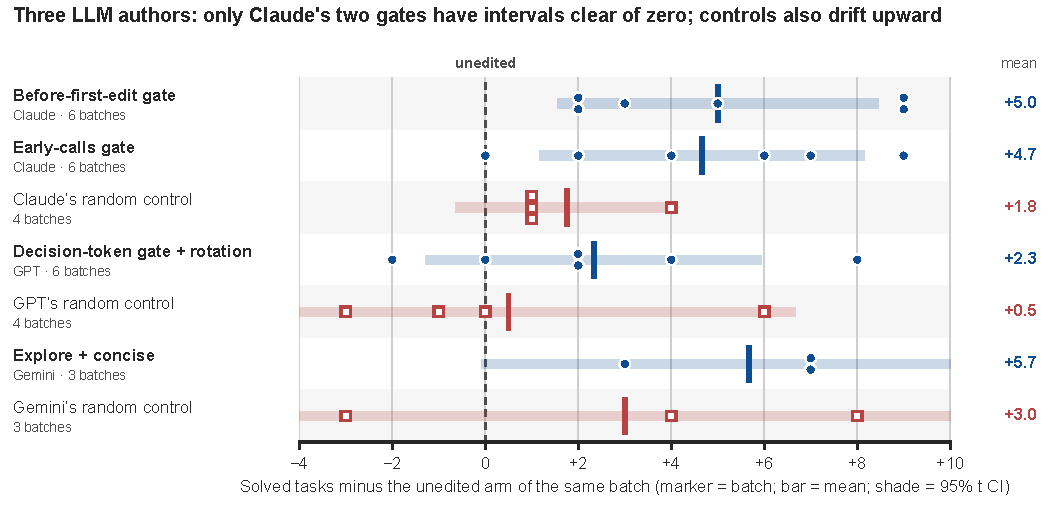
\includegraphics[width=1.0\linewidth]{figures/fig4_arena.pdf}
\end{center}
\caption{\textbf{Three-author benchmark.} Solved tasks of each repeated edit (blue) and each author's random control (red) minus the unedited arm of the same batch; one marker per batch, bar = mean, shade = 95\% $t$ interval of the mean. Only Claude's two gates have intervals that exclude zero, and no edit survives correction for the twelve screened (\S\ref{sec:arena}).}
\label{fig:arena}
\end{figure}

\subsection{Diagnosis tallies}
\label{app:diag}
\textbf{What the brief contained.} The three authors shared one brief. It stated lab-notebook rates for the unedited model and earlier results: 32\% of \texttt{edit\_file} calls fail (an earlier lab-notebook tally from batches 3--5; over the 13 unedited runs below the rate is 35\%); episodes with no failed edit solve 21\% against 4\% with one or more; the $N$th edit of an episode fails 14, 39, 49 and 60\% of the time; how episodes end (tests passed locally 64\%, never edited 17\%, tests errored 16\%); and the solved counts of earlier edits, including always-on explore-more. It gave no odds ratio, no reading-before-editing tally and no tally of calls before the first edit. Neither analysis below was in it. We computed the scripted analysis from a per-episode feature file written on 11 November, before the author sessions. Claude computed its tallies during its session.

\textbf{Scripted analysis} (2,720 episodes: 16 runs of the 170 tasks in batches 3--5, edited arms included; Mantel--Haenszel over tasks). Episodes with any failed edit: 54 of 988 solved against 355 of 1,732 without (odds ratio 0.27, $z = -6.9$, 54 informative tasks). Episodes with a completion of 2,500 tokens or more: 33 of 706 solved against 376 of 2,014 (odds ratio 0.34, $z = -4.6$, 47 tasks). On the three unedited runs alone (510 episodes) these odds ratios are 0.5 and 0.25, and the reading-before-first-edit odds ratio is 1.0.

\textbf{Claude's log} (13 unedited runs of batches 3--15, 2,210 episodes, 342 solved). The authoring model computed these tallies in its session and wrote them to \texttt{diag.log} and \texttt{diag2.log} in its work directory. We recomputed the edit-failure and calls-before-first-edit tallies independently from the saved trajectories and added 95\% intervals (\texttt{diag\_recompute/RESULT.md}). The recomputation reproduces every value, except for two episodes that the author's script put in the wrong failed-edit group. Of 4,916 \texttt{edit\_file} calls, 1,726 fail (35\%; 1,727 in our recomputation, part of the same two-episode discrepancy). The call right after a failed edit is \texttt{read\_file} in 37\% of cases and another \texttt{edit\_file} in 36\%. The next edit of the same file fails 82\% of the time without a re-read ($n = 741$) and 69\% with one ($n = 500$). Within-task odds ratios of solving: any failed edit 0.42; first edit failed 0.57. By number of calls before the first edit, the odds ratios are 0.76 for 0--2 calls, 1.42 for 3--4, 1.72 for 5--7 and 0.12 for 8 or more. Exploring longer is thus not monotonically better. The mean number of calls before the first edit is 4.8. We regenerated this last tally with the author's script (\texttt{diag2.py}) on the same 13 runs. The four bins hold 27\%, 34\%, 22\% and 17\% of episodes. The raw solve rate with versus without each bin is 0.283/0.107, 0.143/0.161, 0.113/0.166 and 0.027/0.181. The raw rate is highest for 0--2 calls because the model edits easy tasks quickly. Within task, the point estimates rise to 5--7 calls and fall at 8 or more; only the 8+ bin's interval excludes 1. The first-edit-failed odds ratio (0.57) and the re-read tallies are the author's values.

\section{What did not work: details}
\label{app:negative}
Each item states what was tried and the measured outcome. Solved counts are out of 170 development tasks, one run per arm, unless stated.

\begin{itemize}
    \item \textbf{Patch correctness is weakly readable.} A class-mean-difference direction for ``the patch being submitted is right'' reaches held-out AUC 0.61--0.62 at layers 24--28 (319 training and 152 held-out decisions per class, split by episode). A paired variant with 83 held-out decisions per class reaches 0.45--0.46. The explore direction reaches 0.77--0.83 by the same method. Writing the 0.61 direction at three strengths solved 30, 25 and 25 against 27 unedited.
    \item \textbf{Test before submitting} (wave-5 adapter) solved 17 against 30 for the adapter without the edit and 30 for its matched random control (Table~\ref{tab:schedule}, batch 4: \texttt{vfyD\_t1.0} against \texttt{w5}). A verify-more edit on the base model solved 24 against 24 unedited (control 27).
    \item \textbf{Submit sooner} (wave-5 adapter) moved behaviour as predicted (\S\ref{sec:control}). It solved 33, 26 and 27 at strengths 0.25, 0.5 and 1.0 against 36 without the edit (Table~\ref{tab:schedule}, batch 5: \texttt{sub\_t}$s$ against \texttt{w5}). Episodes that now submitted in time submitted wrong patches.
    \item \textbf{Think briefly} moved thinking tokens as predicted (\S\ref{sec:control}) and solved 28, 28 and 25 against 29 unedited.
    \item \textbf{Edits aimed at failed file edits.} We tried a gated neuron that reads ``my last edit failed'' and writes ``read the file again'', and a neuron for ``this edit will apply''. Both left the share of regenerated edits whose quoted text exists in the file at 0.65--0.70 across 240 held-out decisions (0.67 unedited; values from the project notes).
    \item \textbf{Compiling a written rule.} Two rules from \S\ref{sec:diagnosis} (``read the relevant code before your first edit''; ``quote the current file text exactly, and re-read after any edit'') solved 25, 29 and 30 (first rule, second rule, both) as prompt text against 30 unedited in one batch. As prompts, they gave no gain. We then compiled each rule into weights (Appendix~\ref{app:rule}). At 400 logged decisions, we ran the model with and without the rule in its prompt and fitted the resulting shift of the layer-18 output. On 88 held-out decisions, a rank-16 compiled edit reproduces 53\% and 41\% of the shift ($R^2$) for the two rules, and one constant neuron reproduces 25\% and 19\%. This experiment tests whether weights can reconstruct a prompt's effect on activations; it does not test whether the rule helps. Ten runs of constant-neuron rule edits in two batches solved 24--31 (mean 27.5) against 28 and 25 unedited (exact McNemar $p \geq 0.36$ for each run; two controls solved 23). An infrastructure failure cut the rank-16 batch (batch 16) short. On the 118 tasks that every arm finished, compiled edits solved 18--22 against 18 unedited and 22 for both controls.
    \item \textbf{Single-run edits in the benchmark.} GPT's re-check-after-error gate ($-2$), rank-two rotation ($-1$) and plain decision-token gate ($-1$) did not beat the unedited model of their batch (Appendix~\ref{app:calib}).
    \item \textbf{High strength.} Always-on explore-more at strength 1.0 solved 18 against 24 unedited (Table~\ref{tab:explore}).
    \item \textbf{One-shot weight deletion.} Deletion Tuning~\citep{Lu2026SurprisingEffectiveness} learns a binary mask over weights by training. We tried a one-shot variant with no optimisation step. One exact REINFORCE gradient over existing rollouts (782) ranks entries of the MLP gate projection by the first-order predicted gain from zeroing them. We restricted the candidates to 16 rows per layer in all 42 layers, so the deletion is a rank-16 LoRA update stacked on the wave-5 RL adapter. Of 1,720,320 candidate entries, 755,581 had positive predicted gain. On one batch of 64 tasks, the adapter without deletion solved 10. Deleting all chosen entries solved 8, and deleting the top 10\% solved 9. Deleting random entries in the same rows with the same counts solved 14 and 12. The gradient-chosen deletions were below both the adapter without deletion and the random deletions. This one-shot first-order variant did not help; the experiment does not test learned masks.
\end{itemize}

\begin{table}[h]
\caption{Episode cost on the 170 development tasks, batches 21--28: mean per episode for the arm and for the unedited model of the same batches; $p$ from a batch-level paired $t$ test. Claude's control is ungated and sized to a 0.125 gap.}
\label{tab:cost}
\centering
\footnotesize
\resizebox{\linewidth}{!}{\begin{tabular}{lrrrrrrr}
\toprule
 & & \multicolumn{3}{c}{Tool calls \dn} & \multicolumn{3}{c}{Seconds \dn} \\
\cmidrule(lr){3-5}\cmidrule(lr){6-8}
Arm & Batches & Arm & Unedited & $p$ & Arm & Unedited & $p$ \\
\midrule
Claude: before-first-edit gate & 6 & 12.03 & 10.61 & 0.008 & 180.6 & 170.8 & 0.055 \\
Claude: early-calls gate & 6 & 12.42 & 10.61 & 0.002 & 185.8 & 170.8 & 0.004 \\
GPT: decision-token gate + rotation & 6 & 10.88 & 10.54 & 0.33 & 168.5 & 165.0 & 0.39 \\
Gemini: explore + concise & 3 & 10.83 & 10.83 & 1.00 & 152.7 & 153.9 & 0.53 \\
Claude's random control & 4 & 11.31 & 10.55 & 0.10 & 180.6 & 179.4 & 0.76 \\
GPT's random control & 4 & 10.63 & 10.45 & 0.37 & 171.0 & 170.7 & 0.91 \\
Gemini's random control & 3 & 10.72 & 10.83 & 0.75 & 158.0 & 153.9 & 0.29 \\
\bottomrule
\end{tabular}}
\end{table}

\begin{figure}[h]
\begin{center}
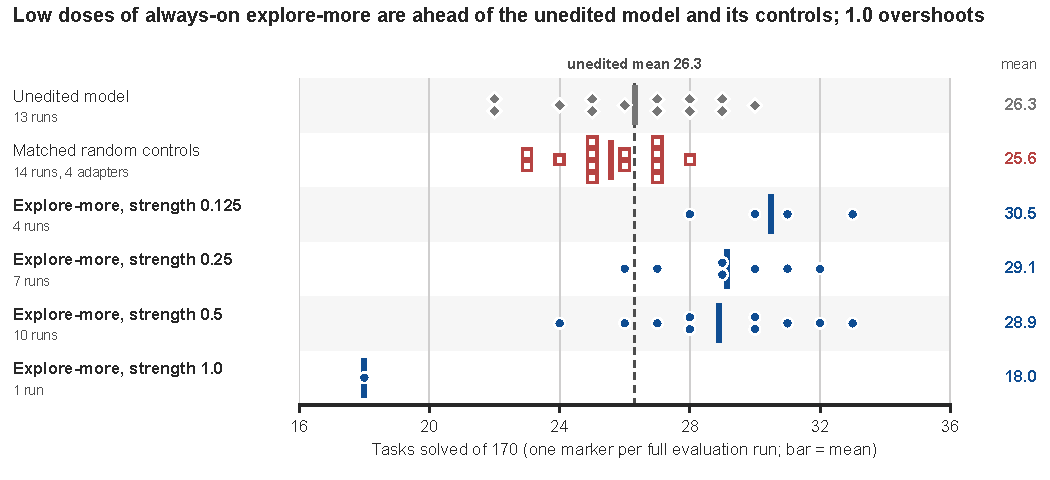
\includegraphics[width=1.0\linewidth]{figures/fig3_solve.pdf}
\end{center}
\caption{\textbf{Always-on explore-more on the development tasks.} Solved tasks of 170 per full evaluation run (one marker per run, bar = mean) for the unedited model (13 runs), matched random-direction controls (14 runs of four adapters) and the edit at four strengths. Strength 1.0 overshoots.}
\label{fig:solve}
\end{figure}

\section{Experiments run after the held-out tests}
\label{app:followup}
We ran these experiments after both held-out tests. None changes a conclusion of the main text.

\subsection{Compiled edit versus an activation hook}
\label{app:hook}
We compare three ways to apply the same edit at the same held-out first-edit decisions. (A) is the compiled adapter as served. (N) is a hook that adds the intended neuron write $\gelu(g \cdot \hat{x})\,(u \cdot \hat{x})\, v$ to the MLP output of the three layers, with $\hat{x}$ the normalised MLP input. (V) is a hook that adds the constant or gate-scaled vector $m\, d_l$ to the layer output, as in activation addition. For the one edited neuron per layer, the adapter stores the edited gate row, up row and down column minus the dequantised 4-bit base weights. It is applied unmerged on top of the 4-bit weights. We run the control the same three ways. For explore-more, this is the matched random control. For the gate, it is Claude's ungated 0.125-gap random control, whose predicted shift is about one-fifth of the gate's. Part~1 teacher-forces the logged completion through a reimplementation of the deployed forward pass (4-bit weights, bfloat16) on 76 decision points. It compares residual changes at all positions and next-token distributions. Part~2 regenerates the decision greedily with the dense checkpoint in a second framework, on 57 points, for always-on explore-more.

\begin{table}[h]
\caption{Compiled adapter (A) against a neuron-write hook (N) and a vector-addition hook (V); mean over 76 held-out decision points. Cosines and $R^2$ compare the change from the unedited model in the residual stream at the stated layer; intervals on the cosines are within $\pm 0.003$.}
\label{tab:hook}
\centering
\small
\resizebox{\linewidth}{!}{\begin{tabular}{lrr}
\toprule
 & Explore-more 0.25 & Before-first-edit gate \\
\midrule
Cosine A vs N, layers 18 / 22 / 41 \up & 0.992 / 0.992 / 0.972 & 0.994 / 0.996 / 0.984 \\
Norm ratio A / N, layer 41 & 1.001 & 1.000 \\
$R^2$ A vs N, layers 18 / 41 \up & 0.984 / 0.945 & 0.989 / 0.968 \\
Cosine A vs V, layers 18 / 22 / 41 & 0.949 / 0.804 / 0.946 & 0.955 / 0.731 / 0.945 \\
Cosine A vs control, layer 41 & 0.056 & 0.018 \\
Projection on write direction$^{b}$ / class gap, layer 18: A / N / V & 0.236 / 0.236 / 0.250 & 0.249 / 0.249 / 0.265 \\
KL(unedited $\Vert$ A), completion tokens & 0.0112 & 0.0127 \\
KL(unedited $\Vert$ A), decision position & $3.4\times10^{-5}$ & $3.4\times10^{-5}$ \\
KL(N $\Vert$ A) \dn & 0.00011 & 0.00012 \\
KL(V $\Vert$ A) \dn & 0.00039 & 0.00051 \\
KL(unedited $\Vert$ control)$^{a}$ & 0.0029 & 0.0056 \\
\bottomrule
\end{tabular}}

\smallskip
\raggedright\footnotesize $^{a}$ Gate column: Claude's ungated 0.125-gap control. It writes at every position, unlike the gate, so it is not gate-matched. KL rows are over the positions that predict completion tokens (about 870 per point) unless marked ``decision position''. $^{b}$ The unit direction that the edit writes along at that layer, not the signed class direction $d$, so a positive value is a shift in the intended sense.
\end{table}

The compiled adapter reproduces the hooked neuron write. Its next-token distribution is about 100 times closer to the hook's than to the unedited model's (Table~\ref{tab:hook}). A plain vector addition is a looser match, most visibly at layer 22 (cosine 0.80 and 0.73). At the decision position itself, the gate's adapter--hook cosine at layer 18 is 0.883 (one point at 0.044). The output distributions there still agree closely (gate: KL(N$\,\Vert\,$A) $7.9\times10^{-7}$ against KL(unedited$\,\Vert\,$A) $3.4\times10^{-5}$). At the decision position, the edits' own KL ($3.4\times10^{-5}$ for both) is about 330 to 370 times smaller than over the completion tokens (0.0112 and 0.0127). Regeneration covered 57 points for always-on explore-more only, too few to detect the edit's own effect, and it does not separate the adapter from either hook. Over these 57 points, the share of decisions that are edits is 0.632 unedited, 0.614 for A, 0.544 for N and 0.632 for V. The difference N minus A is $-0.070$ (95\% CI $-0.153$ to $+0.013$). N agrees with A on the tool chosen at 86\% of points, close to the unedited model's 88\%. On these 57 points the edit itself does not move the edit share (A minus unedited $-0.018$, CI $-0.109$ to $+0.074$), so this part does not rank the three. The two hooks differ from each other (N minus V $-0.088$, CI $-0.162$ to $-0.014$, uncorrected over 24 comparisons: 12 pairs, two metrics). The hooks reproduce the adapter's full output on 5 of 57 points, against 0 of 57 for the unedited model.

\textbf{Setup notes.} Part~1 covers 76 of the 320 planned points and runs in one framework. The 57 points of Part~2 are the 27 longest and 30 shortest prompts of the first 104. The hook adds in bfloat16. A replaces the overwritten neuron, while N adds a new neuron beside it. The remaining difference between A and N ($1 - R^2$ of 0.8 to 5.5\%, growing with depth) therefore combines the old neuron's output and numerical precision. Regeneration uses HF transformers with dense bfloat16 weights, which are identical to the dequantised 4-bit weights. In that framework the explore-more edit's decision-position KL between unedited model and adapter has mean 0.0065 over the 57 points (heavy-tailed), against $3.4\times10^{-5}$ in Part~1. For the gate's control, the vector hook (CV) matches the control adapter (C) poorly: the cosine between their residual changes is 0.12 at layer 18 and 0.42 at layer 20, and the adapter's change is about 7 and 2 times the hook's in norm. This control is ungated with a small intended shift (0.02 to 0.05 class gaps, against about 0.26 for the gate), so most of its adapter's change at these layers lies off the added vector. Its neuron hook still matches it (cosine 0.96 to 0.99). We ran regeneration for explore-more only.

\subsection{Round 2: dose, depth and gate variants of the before-first-edit gate}
\label{app:round2}
One author (Claude) built variants of its before-first-edit gate. We ran them in two batches, each with its own unedited arm. Table~\ref{tab:round2} lists every arm.

\begin{table}[h]
\caption{Round 2, 170 development tasks, one run per arm. ``Better / worse'' counts tasks solved by the arm and not by the unedited model of the same batch, and the reverse; $p$ is a two-sided sign test. Strength is in class gaps. One arm was stopped early.}
\label{tab:round2}
\centering
\small
\resizebox{\linewidth}{!}{\begin{tabular}{llrrrr}
\toprule
Batch & Arm & Solved \up & Unedited & Better / worse & $p$ \\
\midrule
29 & Before-first-edit gate, 0.25 (repeat) & 28 & 25 & 12 / 9 & 0.66 \\
29 & Same gate on five layers (16--24) & 28 & 25 & 13 / 10 & 0.68 \\
29 & Gate + layers 24--28 of Gemini's explore + concise edit & 28 & 25 & 10 / 7 & 0.63 \\
29 & Gate at strength 0.5 & 25 & 25 & 8 / 8 & 1.00 \\
29 & Gate at strength 1.0 (stopped at 96 tasks) & 2 of 96 & & & \\
\midrule
30 & Gate 0.25 + early-calls gate 0.3 & 33 & 28 & 13 / 8 & 0.38 \\
30 & Early-calls gate at strength 0.6 & 30 & 28 & 8 / 6 & 0.79 \\
30 & Early-calls gate (round-1 edit, repeat) & 28 & 28 & 9 / 9 & 1.00 \\
30 & Gate 0.5 + layers 24--28 of Gemini's edit & 21 & 28 & & \\
30 & Five-layer gate at strength 0.5 & 12 & 28 & & \\
\bottomrule
\end{tabular}}
\end{table}

A higher dose did not help. Strength 0.5 matched the unedited model on three layers and lost 16 tasks on five layers. Strength 1.0 solved 2 of its first 96 tasks. The best arm, the gate combined with the early-calls gate, was 5 tasks ahead in its one batch. This difference is within the spread of single batches.

\subsection{Round 3: stacking edits from different authors}
\label{app:round3}
We wrote predictions and a decision rule before any run. A stacked edit goes to a new held-out test only if it beats the unedited model by at least 8 tasks in the mean of two batches and by at least 5 in each, and beats a stacked control by at least 5.

\textbf{A plain sum of adapters is not a stack.} The authors' builders all overwrite the quietest neurons of a layer, so their edits share neurons. For example, every edit uses neuron 2972 of layer 20. A sum of two adapters therefore gives one neuron with mixed gate, up and down weights, not two neurons. With such sums, every stacked arm, the stacked control included, ended every episode without a submission. We stopped that batch after 3 to 18 tasks per arm and use none of its numbers. We rebuilt the stacks so that a later source's neuron moves to the next quietest free neuron of the layer and carries the source's exact edited weights.

\textbf{Result.} We stopped the two batches with the rebuilt stacks at 49 to 106 of 170 tasks per arm, so the decision rule is not evaluated. Table~\ref{tab:round3} gives the counts on the tasks completed by both an arm and the unedited model of its batch. Before this intersection, the unedited arm had completed 106 tasks in batch 33 and 82 in batch 34, and the other arms 56 to 106 and 49 to 84. The largest difference for a stack is $+3$ tasks over the two batches (gate plus Gemini's edit, 26 against 23). The stacked control is $+2$ (29 against 27). The other two stacks are behind (21 against 23, and 15 against 16). The repeat of the best round-2 arm is level with the unedited model (25 against 24 over the two batches).

\begin{table}[h]
\caption{Round 3: solved tasks among those completed by both the arm and the unedited model of the same batch (batches 33 and 34). The pre-registered rule needs complete batches and is not evaluated. The intersections (49 to 106 tasks) favour tasks that finish quickly and differ between arms.}
\label{tab:round3}
\centering
\small
\begin{tabular}{lrrrrrr}
\toprule
 & \multicolumn{3}{c}{Batch 33} & \multicolumn{3}{c}{Batch 34} \\
\cmidrule(lr){2-4}\cmidrule(lr){5-7}
Arm & Tasks & Arm & Unedited & Tasks & Arm & Unedited \\
\midrule
Gate + Gemini's explore-and-concise edit & 94 & 14 & 12 & 73 & 12 & 11 \\
Gate + early-calls gate + Gemini's edit & 83 & 12 & 12 & 73 & 9 & 11 \\
Same, writes scaled by 0.7 & 56 & 8 & 9 & 49 & 7 & 7 \\
Stacked control & 106 & 14 & 14 & 82 & 15 & 13 \\
Gate + early-calls gate (round-2 best, repeat) & 93 & 14 & 12 & 77 & 11 & 12 \\
\bottomrule
\end{tabular}
\end{table}

\subsection{Round 4: a wide screen motivated by the loss after long exploration}
\label{app:round4}
\textbf{Design, fixed before launch} (\texttt{round4\_predictions.md}, with six dated amendments). We wrote each amendment before the decision-rule batches were scored. Amendments 3 and 5 record partial scores of the batches they stop (b35 on 41 tasks, b46 on 57; 42 and 59 in the final logs, with the same conclusions). The diagnosis of \S\ref{sec:diagnosis} shows that episodes with 8 or more calls before the first file edit solve far less (odds ratio 0.12). The point estimates peak at 5--7 calls; that bin's interval includes 1. Earlier edits pushed only towards more exploration. Round 4 adds a ``commit late'' neuron that pushes towards the first edit once 8 or more calls have passed without one. We test it alone (\texttt{late30}, \texttt{late60}) and combined with the early explore push (\texttt{u*}, \texttt{pu}). We also test dose, depth and gate variants of the before-first-edit gate (\texttt{pe*}, \texttt{pre*}) and two random-direction family controls. This gives 20 adapters in four arm sets of five. Each batch has its own unedited arm, 170 development tasks and one rollout. Each edit has a written prediction: an interval of solved tasks relative to the unedited arm of its batch. Decision rule: an edit goes to a held-out test only if its mean gain over its two batches is at least 8 tasks, it gains at least 5 in each batch, and its mean gain exceeds its family control's by at least 5. We screen twenty edits, so any development $p$ value is Holm-corrected over 20. A secondary pooled analysis (per-edit paired difference summed over all its batches, task-level sign test, Holm over 20) is reported but cannot send an edit to a held-out test.

\textbf{Protocol notes.} Six of the first eight batches were relaunched within 20 minutes under new batch names to fit sandbox capacity. Batches that stopped before 170 tasks are scored on the tasks completed by every arm and marked incomplete. Batches ran at concurrency 4 per arm (35, 36, 45, 46), 6 (43, 44) or 8 (47--58). Every arm of a batch shares its setup, and we compare each edit only with the unedited arm of its own batch. Episodes have a 7.5-minute wall-clock limit, and we count session-limit rows per arm (Tables~\ref{tab:round4b} and~\ref{tab:round4}). Amendment~3 named batch 36 a decision-rule batch before it was scored, so we keep it at 156 tasks. That amendment replaced batch 35 with batch 45. Batch 46 was a third batch outside the rule. For the explore-plus-commit-late set (\texttt{u33}, \texttt{u36}, \texttt{u63}, \texttt{u33\_L5}, \texttt{u33\_c6}) and the depth and dose set (\texttt{pe\_L*}, \texttt{pre15}, \texttt{pre35}), the family control ran in a different batch. For these two sets, rule~3 compares across batches.

\textbf{Results.} No edit passes the pre-registered rule. In the first batch of each arm set (Table~\ref{tab:round4}), the best edits gained 5 tasks (two edits), and 6 in batch 36, against the rule's 8. No single-batch difference has $p < 0.17$ except one failure. The depth variant that writes at layer 14 solved 1 of 170 tasks in both batches (0 won and 22 lost in batch 44, 0 and 28 in batch 50): this edit breaks the model at that depth. The largest single-batch gain, $+7$, belongs to a random-direction control (\texttt{u33\_ctrl}, batch 36). The explore-gate family's control lost 4 in batch 43. Under the decision rule, each edit has two batches (first arm set: 45 and 47; second: 36 and 48; third: 43 and 49; fourth: 44 and 50; Table~\ref{tab:round4b} and Figure~\ref{fig:round4}). The best mean gains are $+5.0$ for \texttt{pe\_L5} ($+5$, $+5$), \texttt{pe\_lo} ($+4$, $+6$) and \texttt{u36} ($+1$, $+9$; the $+9$ has uncorrected $p = 0.049$), and $+4.5$ for \texttt{pe\_L20} ($+1$, $+8$). None reaches the required $+8$, so no edit passes and none goes to a held-out test. Most edited arms have more session-limit rows than the unedited arm of the same batch (for example \texttt{pe\_hi} 28 against 14 and \texttt{u33\_ctrl} 26 against 13 in Table~\ref{tab:round4b}). For 10 of the 20 adapters, the written interval (mean width 4.05 tasks) contains the measured two-batch mean. There are 5 misses above and 5 below; the largest is \texttt{pe\_L14}, $-25$ against 0 to $+3$. Two intervals stated relative to a three-layer version are resolved against its measured mean. Of the 40 single batches, 18 fall inside their intervals. The secondary pooled analysis (Amendment 4) sums each edit's paired differences over every batch it ran in, the replicate batches 51--58 included. It applies a task-level sign test with Holm correction over the 20 adapters. The largest pooled gain is \texttt{pe\_lo}: 39 tasks won and 17 lost over 678 task pairs ($+22$, $p = 0.005$, Holm-adjusted $p = 0.087$; \texttt{pe\_L14} has the smallest $p$, so the step-down multiplies \texttt{pe\_lo}'s $p$ by 19 of the 20). This gain does not survive correction. The next are \texttt{pe\_L20} $+15$ ($p = 0.086$), \texttt{pe\_L5} $+13$ ($p = 0.12$), \texttt{pe\_c6} $+10$ and the random-direction control \texttt{u33\_ctrl} $+10$. No adapter is significant after correction. The pooled analysis uses the replicate batches as of 4:27 PM ET (batch 58 at 103--110 tasks); it does not affect the decision-rule verdict. Round 6 (Appendix~\ref{app:round6}) is the pre-registered replication of \texttt{pe\_lo}.

\begin{table}[h]
\caption{Round 4, second batch of each arm set (batches 47--50, all complete): solved tasks against the unedited arm of the same batch; won / lost are discordant tasks; the last column counts rows that ended at the 7.5-minute session limit for the unedited arm / the edit.}
\label{tab:round4b}
\centering
\small
\begin{tabular}{llllrrrr}
\toprule
Batch & Tasks & Arm & Unedited & Arm & $\Delta$ & Won / lost & Limit rows \\
\midrule
47 & 170 & \texttt{u33} & 24 & 26 & +2 & 10 / 8 & 15 / 20 \\
47 & 170 & \texttt{u33\_L5} & 24 & 29 & +5 & 14 / 9 & 15 / 23 \\
47 & 170 & \texttt{u33\_c6} & 24 & 29 & +5 & 12 / 7 & 15 / 23 \\
47 & 170 & \texttt{u36} & 24 & 33 & +9 & 13 / 4 & 15 / 24 \\
47 & 170 & \texttt{u63} & 24 & 28 & +4 & 13 / 9 & 15 / 16 \\
\midrule
48 & 170 & \texttt{pre\_early} & 25 & 27 & +2 & 8 / 6 & 13 / 23 \\
48 & 170 & \texttt{late30} & 25 & 27 & +2 & 9 / 7 & 13 / 18 \\
48 & 170 & \texttt{late60} & 25 & 25 & 0 & 6 / 6 & 13 / 22 \\
48 & 170 & \texttt{pu} & 25 & 22 & $-3$ & 7 / 10 & 13 / 22 \\
48 & 170 & \texttt{u33\_ctrl} (control) & 25 & 26 & +1 & 9 / 8 & 13 / 26 \\
\midrule
49 & 170 & \texttt{pe\_L5} & 24 & 29 & +5 & 11 / 6 & 14 / 21 \\
49 & 170 & \texttt{pe\_c6} & 24 & 29 & +5 & 10 / 5 & 14 / 14 \\
49 & 170 & \texttt{pe\_ctrl} (control) & 24 & 24 & 0 & 6 / 6 & 14 / 20 \\
49 & 170 & \texttt{pe\_hi} & 24 & 27 & +3 & 9 / 6 & 14 / 28 \\
49 & 170 & \texttt{pe\_lo} & 24 & 30 & +6 & 10 / 4 & 14 / 13 \\
\midrule
50 & 170 & \texttt{pe\_L14} & 29 & 1 & $-28$ & 0 / 28 & 16 / 5 \\
50 & 170 & \texttt{pe\_L20} & 29 & 37 & +8 & 15 / 7 & 16 / 19 \\
50 & 170 & \texttt{pe\_L22} & 29 & 25 & $-4$ & 6 / 10 & 16 / 25 \\
50 & 170 & \texttt{pre15} & 29 & 27 & $-2$ & 6 / 8 & 16 / 15 \\
50 & 170 & \texttt{pre35} & 29 & 26 & $-3$ & 6 / 9 & 16 / 23 \\
\bottomrule
\end{tabular}
\end{table}

\begin{figure}[h]
\begin{center}
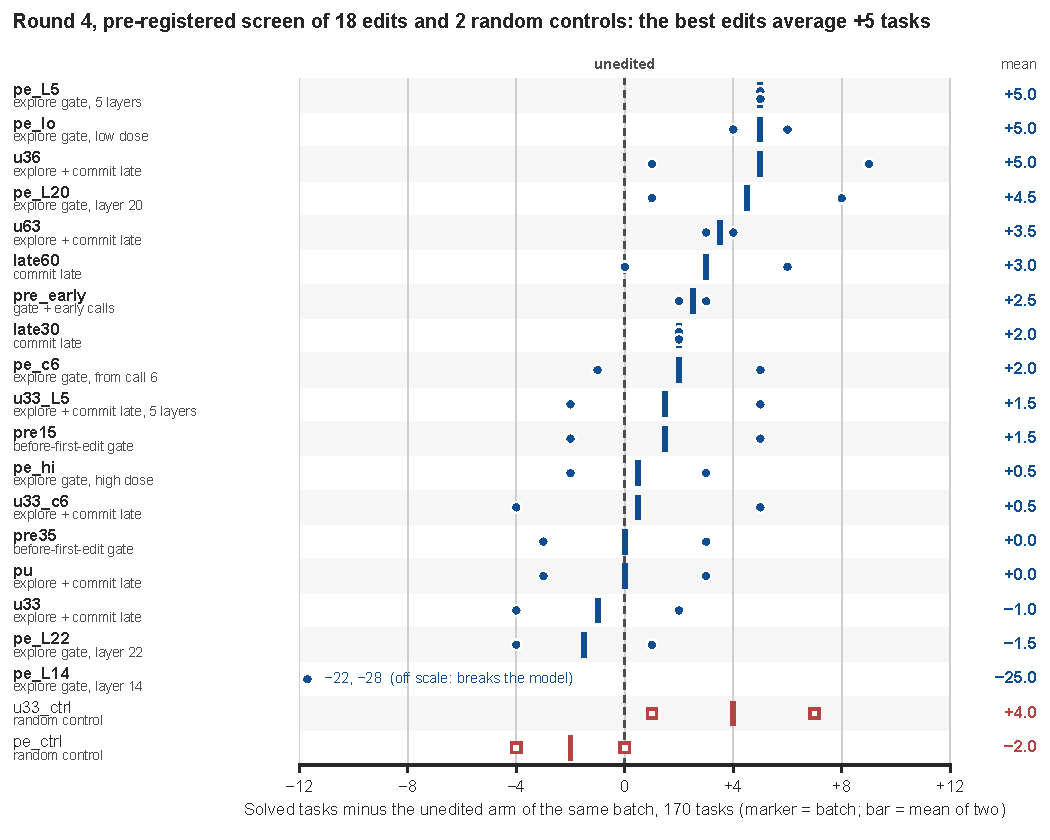
\includegraphics[width=1.0\linewidth]{figures/fig6_round4.pdf}
\end{center}
\caption{\textbf{Round 4: no edit reaches the pre-registered bar.} Each of the 18 edits and two random-direction controls in its two batches (first batch: 45, 36 [stopped at 156 tasks], 43 or 44; second: 47--50), as solved tasks minus the unedited arm of the same batch; bar = mean of the two. The pre-registered rule required a mean of at least $+8$, at least $+5$ in each batch and $+5$ over the family control. The layer-14 variant solved 1 of 170 in both batches (off scale).}
\label{fig:round4}
\end{figure}


\begin{table}[h]
\caption{Round 4, first batch of each arm set: solved tasks on the tasks completed by every arm of the batch, each arm against the unedited arm of its own batch; won / lost are discordant tasks, $p$ an exact two-sided sign test (shown when below 0.5). Batch 36 was stopped at 156 tasks complete in every arm (Amendment 6; arms had completed 158 to 166). Batches 35 (42 common tasks; arms 42 to 52) and 46 (59; arms 59 to 70) were stopped early and are not tabulated; intersections of stopped batches favour tasks that finish quickly: in batch 35 every arm was within $-1$ to $+2$ of the unedited model (6 solved), and in batch 46 the arms solved 7 to 12 against 10. The last column counts rows that ended at the 7.5-minute session limit, unedited arm / edit (batch 36 from the final logs, which have 157 common tasks: one more task finished in every arm after the stop and no arm solved it, so solved counts and won / lost are those at 156).}
\label{tab:round4}
\centering
\small
\resizebox{\linewidth}{!}{\begin{tabular}{lllrrrrrr}
\toprule
Batch & Status & Arm & Unedited & Arm & $\Delta$ & Won / lost & $p$ & Limit rows \\
\midrule
43 & complete & \texttt{pe\_L5} & 28 & 33 & +5 & 10 / 5 & .30 & 10 / 17 \\
43 & complete & \texttt{pe\_lo} & 28 & 32 & +4 & 9 / 5 & .42 & 10 / 13 \\
43 & complete & \texttt{pe\_c6} & 28 & 27 & $-1$ & 7 / 8 &  & 10 / 21 \\
43 & complete & \texttt{pe\_hi} & 28 & 26 & $-2$ & 5 / 7 &  & 10 / 23 \\
43 & complete & \texttt{pe\_ctrl} (control) & 28 & 24 & $-4$ & 3 / 7 & .34 & 10 / 26 \\
\midrule
44 & complete & \texttt{pre15} & 23 & 28 & +5 & 9 / 4 & .27 & 10 / 12 \\
44 & complete & \texttt{pre35} & 23 & 26 & +3 & 8 / 5 &  & 10 / 18 \\
44 & complete & \texttt{pe\_L20} & 23 & 24 & +1 & 8 / 7 &  & 10 / 17 \\
44 & complete & \texttt{pe\_L22} & 23 & 24 & +1 & 10 / 9 &  & 10 / 15 \\
44 & complete & \texttt{pe\_L14} & 23 & 1 & $-22$ & 0 / 22 & $<$.001 & 10 / 4 \\
\midrule
45 & complete & \texttt{u63} & 27 & 30 & +3 & 11 / 8 &  & 2 / 4 \\
45 & complete & \texttt{u36} & 27 & 28 & +1 & 7 / 6 &  & 2 / 4 \\
45 & complete & \texttt{u33\_L5} & 27 & 25 & $-2$ & 6 / 8 &  & 2 / 1 \\
45 & complete & \texttt{u33} & 27 & 23 & $-4$ & 9 / 13 &  & 2 / 3 \\
45 & complete & \texttt{u33\_c6} & 27 & 23 & $-4$ & 7 / 11 &  & 2 / 5 \\
\midrule
36 & 156 tasks & \texttt{u33\_ctrl} (control) & 22 & 29 & +7 & 13 / 6 & .17 & 14 / 13 \\
36 & 156 tasks & \texttt{late60} & 22 & 28 & +6 & 11 / 5 & .21 & 14 / 14 \\
36 & 156 tasks & \texttt{pre\_early} & 22 & 25 & +3 & 10 / 7 &  & 14 / 17 \\
36 & 156 tasks & \texttt{pu} & 22 & 25 & +3 & 10 / 7 &  & 14 / 13 \\
36 & 156 tasks & \texttt{late30} & 22 & 24 & +2 & 10 / 8 &  & 14 / 18 \\
\bottomrule
\end{tabular}}
\end{table}


\subsection{Round 5: dose and timing ladder of the commit-late edit (exploratory)}
\label{app:round5}
Round 5 is one exploratory batch with eight arms. We wrote predictions and a pass rule before launch (\texttt{round5\_predictions.md}). The arms are: the round-4 \texttt{late60} edit as anchor; a larger target (0.9 class gaps); fixed 3$\times$ and 5$\times$ multiples of the \texttt{late60} write sizes; two variants that push from call 6; a random-direction control matched to \texttt{late60}; and the unedited model. Class-gap targets of 1.2 and 2.0, and a five-layer variant (layers 16--24), could not be built. The shift saturated under the RMS normalisation of the MLP output at layer 22 (and at layers 16 and 24), so the solver ran to its cap (write size about 1000). We discarded those builds before serving and used the fixed multiples instead. We stopped the batch at 3:34 PM ET to free capacity for round 6 and score it on the tasks finished by every arm. The arms had completed 52 to 84 tasks, and the 52-task intersection favours tasks that finish quickly. On these 52 tasks the unedited model solved 10 and the \texttt{late60} anchor 8. Its 3$\times$ and 5$\times$ multiples solved 7 and 6. The call-6 variants solved 9 (target 0.6) and 5 (target 1.0). The larger target 0.9 solved 8, and the matched random control 11. A stronger or earlier commit-late push solved fewer tasks, and the control did best. The written intervals (for 170 tasks) contain the measured difference for 3 of the 7 arms: the 3$\times$ and 5$\times$ multiples and the control. The other four push arms fell below their intervals.

\subsection{Round 6: a pre-registered replication of one round-4 edit}
\label{app:round6}
\textbf{Design, fixed before launch} (\texttt{round6\_predictions.md}). We selected one edit from the round-4 data: the low-dose explore gate \texttt{pe\_lo}. It led the interim pooled round-4 analysis, in which no edit met the round-4 rule or survived Holm correction over 20. Round 6 runs \texttt{pe\_lo}, its matched random-direction control and the unedited model in new batches of the same 170 development tasks. Each batch has one rollout and its own unedited arm. Incomplete batches are scored on the tasks finished by all three arms. Primary test, one hypothesis: \texttt{pe\_lo} against the unedited arm of the same batch, task-level paired, exact two-sided sign test on discordant pairs over round-6 episodes only, $\alpha = 0.05$. Prediction: $+2$ to $+7$ tasks per complete batch; control $-3$ to $+2$. The tasks are those on which we selected the edit, so a pass shows that the development gain replicates in fresh episodes. It does not test generalisation to new tasks.

\textbf{Results} (\texttt{r6\_final\_all.txt}, \texttt{r6\_final\_lo\_vs\_ctrl.txt}, \texttt{r6\_final\_no66\_71.txt}). Twenty batches entered the primary test (b60--b71, b73--b80); three ran all 170 tasks (b60, b61, b65), and the rest are scored on the tasks every arm finished. Pooled over 1,930 task pairs, \texttt{pe\_lo} solved 297 against 271 for the unedited model: 105 tasks won and 79 lost, $+26$ net ($+2.3$ per 170 tasks), exact sign test $p = 0.065$. The primary test therefore does not reach the pre-registered $\alpha = 0.05$. In the three complete batches the edit gained $+4$, $+3$ and $+6$, inside the predicted $+2$ to $+7$. The pre-registered sensitivity check without the six batches stopped early (b66--b71) gives $+30$ net over 1,652 pairs (92 won, 62 lost, $p = 0.019$). The random control fell below the unedited model ($-36$ net over 1,847 pairs, 57 won and 93 lost, $p = 0.004$; $-2$, $-5$ and $0$ in the complete batches against a predicted $-3$ to $+2$), so the edit's lead over its control ($+58$ net over 1,836 pairs, 109 won and 51 lost, $p < 0.001$) is larger than its lead over the unedited model. The control also hit the session limit more often (329 rows against 217 for the unedited arm and 204 for the edit), so part of the edit's lead over the control reflects the control's time-outs. In the exploratory batch b72 (Amendment 1), \texttt{pe\_L20} solved 28 and \texttt{pe\_L5} 29 against 29 for its unedited arm ($-1$ and $0$), both below the predicted $+1$ to $+6$.

\subsection{Round 7: an exploratory screen of scaled copies and stacks}
\label{app:round7}
Round 7 tested 28 edits and two random controls built only from existing edits: dose-scaled copies, stacks on separate neurons, and stacks with Gemini's benchmark edits. Each ran in one batch of five arms with its own unedited arm (six batches). The plan and rule were written before any episode (\texttt{round7\_predictions.md}): the round selects nothing, and a gain of $+10$ in a batch would only trigger a rerun. We stopped all batches at 6:00 PM ET and score each on the tasks every arm finished (87--136 tasks). No arm reached $+10$. The largest gain was $+5$ (27 against 22 on 132 tasks) for \texttt{pe\_lo} stacked with a Gemini edit. Six arms were ahead of their unedited arm by 1 to 5 tasks, one was level and 23 were behind; two stacks solved no task. Edited arms hit the session limit more often than the unedited arms (up to 52 rows against 2 to 12), most of all the down-scaled copies. Those copies were repacked as rank-32 adapters without checking that the repack reproduces the source edit, so this round shows that the edits did not help in this form, not a dose-response (\texttt{r7/r7\_summary\_from\_session.txt}).


\end{document}
